\documentclass[../full_thesis/full_thesis.tex]{subfiles}

% Default image directory
\newcommand{\thisdir}{../inertial_frame}
\graphicspath{{\thisdir/img/}}


\begin{document}

In Sec.~\ref{sec: rotating frame} we developed our intuition for the precession
of neutron stars by working in the rotating frame of the star. However, pulsar
astronomers report on direct observations of the radio pulsations in the
inertial frame. In this section, we will develop our precession model by making
predictions for how precession manifests in the observable features of a
pulsar. This will require us to understand and model the data collection
methods of pulsar astronomy. We will study each `physical observable'
separately and discuss how exact numerical results can be computed and derive
analytic approximations. \citet{Ruderman1970} first investigated phase modulation
due to precession, since then there has been extensive work in the literature:
\citet{Nelson1990} calculated phase residuals both analytically
and numerically for freely precessing stars; torqued precession was considered
for a general torque by \citet{Jones1988excitation} and \citet{Cordes1993} and
then for the \citet{Deutsch1955} torque by \citet{Melatos1999, Melatos2000}. In this work,
we will closely follow the analytic results of \citet{Jones2001}. The novel
material here is in developing a numerical solution which allows direct
prediction of the physical observable features measured by observers, even
modelling the data collection mechanisms such as the observer-method to measure
$\dot{\nu}$. This chapter has two important aims: first, we want to develop our
intuition for precession which will be used in Chapter.~\ref{sec: testing
models}; second, this numerical model allows us to add physics into the model and
directly under the predictions it makes for observations. To demonstrate this,
we finish the chapter by showing some preliminary results of a model in which
the EM torque undergoes switching events as suggested by \citet{Lyne2010}.

\section{Rotating into the inertial frame}

\subsection{Euler rotation matrices}
\label{sec: euler rotation matrices}
The Euler rigid body equation of Eqn.~\eqref{eqn: eom} is defined in the
rotating frame of the star. To discuss results in the inertial frame of an
observer, we need to transform the solutions of Euler's rigid body equations
into the inertial frame.  An efficient way to do this is to determine the three
Euler angles which transform the rotating frame axes, denoted by $(x',y',
z')$, to the inertial frame axis, denoted by $(x, y, z)$. In particular, we
define three rotation matrices
\begin{align}
\begin{split}
D = \left[\begin{array}{ccc}
\cos\phi & \sin\phi & 0 \\
-\sin\phi & \cos\phi & 0 \\
0 & 0 & 1
\end{array}
\right],
\\
C =
\left[\begin{array}{ccc}
1 & 0 & 0 \\
0 & \cos\theta & \sin\theta \\
0 & -\sin\theta & \cos\theta
\end{array}
\right], \\
B = \left[\begin{array}{ccc}
\cos\psi & \sin\psi & 0 \\
-\sin\psi & \cos\psi & 0 \\
0 & 0 & 1
\end{array}
\right].
\end{split}
\end{align}
Then their product defines the Euler angle rotation matrix
\begin{align}
\begin{split}
R(\theta, \phi, \psi) & = BCD \\
& \left[
\begin{array}{ccc}
\cos\psi \cos\phi - \cos\theta \sin\phi \sin \psi &
\cos\psi \sin \phi + \cos\theta \cos \psi \sin \psi &
\sin \psi \sin\theta \\
-\sin\psi \cos\phi - \cos\theta\sin\phi\cos\psi &
-\sin\psi\sin\phi + \cos\theta\cos\phi\cos\psi &
\cos\psi \sin\theta \\
\sin\theta\sin\phi &
-\sin\theta \cos\phi &
\cos\theta
\end{array}
\right].
\end{split}
\label{eqn: rotation matrix}
\end{align}
Here we are using the
$(\phi, \theta, \psi)$ Euler
angle parameterisation as described by \citet{Landau1969}; a diagram of how
these angles is given in Fig.~\ref{fig: Euler}.\begin{figure}[ht]
\centering
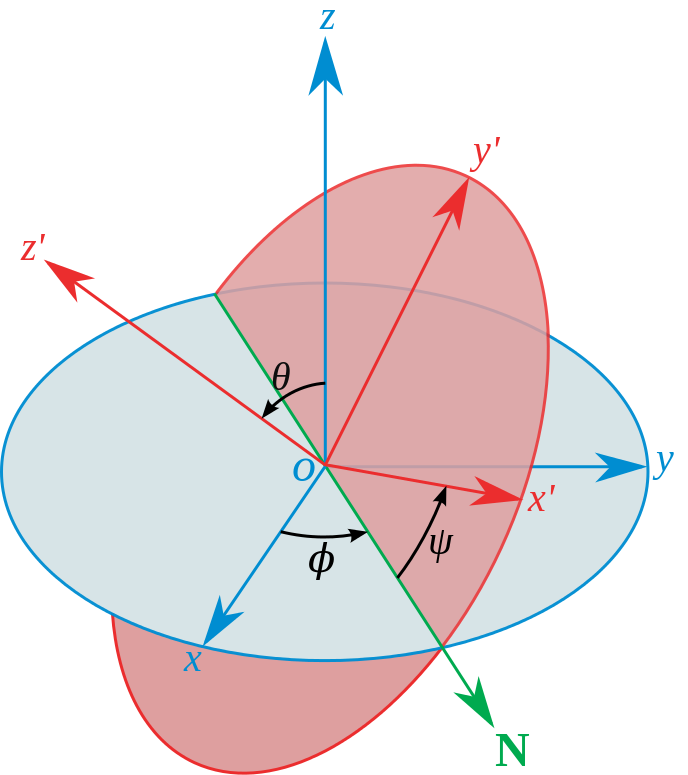
\includegraphics[scale=0.25]{Eulerangles-alternative_filled.png}
\caption{Schematic of the Euler rotation angles between the rotating
frame $(x', y', 'z')$ and the inertial frame $(x, y, z)$. Image courtesy of
 \citet{WikipediaEuler}.}
\label{fig: Euler}
\end{figure}
This matrix, given values for the Euler angles, transforms from the fixed
interial system of coordinates to the rotating frame. So for $A^{\textrm{in}}$,
a vector defined in the inertial frame, in the rotating frame this has
components given by
\begin{align}
A^{\textrm{rot}}_{a} = R^{b}_{\;\;a} A^{\textrm{in}}_{b}.
\end{align}

\subsection{Evolution of the Euler angles}
The Euler angles themselves will evolve with time. To calculate this, we express
the components of $\Omega$ along the moving axes ($x', y', z')$. As shown by
\citet{Landau1969} this results in a set of three ODEs which are coupled both to
the other Euler angles and the components of the spin-vector. To have solutions
both for the motion of the spin-vector in the rotating frame and the Euler
angles we need to solve all six ODEs together. To be specific, the six ODEs are
given in equations~\eqref{eqn: ODEs}: in the left-hand triplet is the
components of the Euler rigid body equations first given in Eqn.~\eqref{eqn:
eom}; in the right-hand triplet we give the rearranged set of Euler angles ODEs
from \citet{Landau1969}.
\begin{align}
\begin{split}
\dot{\omega}_{x} & = \frac{1}{I_{xx}}\left[T_{x} +
                      \left(I_{yy} - I_{zz}\right) \omega_{y} \omega_{z}\right],
\\
\dot{\omega}_{y} & = \frac{1}{I_{yy}}\left[T_{y} +
                      \left(I_{zz} - I_{xx}\right) \omega_{x} \omega_{z}\right],
\\
\dot{\omega}_{z} & =\frac{1}{I_{zz}}\left[T_{z} +
                      \left(I_{xx} - I_{yy}\right) \omega_{x} \omega_{y}\right],
\end{split}
\begin{split}
\dot{\phi} & = \frac{\omega_{x} \sin \psi + \omega_{y} \cos \psi}{\sin \theta},\\
\dot{\theta} & = \omega_{x} \cos \psi - \omega_{y} \sin \psi,\\
\dot{\psi} & = \omega_{z} - \dot{\phi} \cos \theta.
\end{split}
\label{eqn: ODEs}
\end{align}
This set of six coupled ODEs can be solved numerically using a time stepper; we
will use the \texttt{rkf45} stepper provided by GSL \citep{gough2009gnu}.
Solutions give the components of the spin-vector in the rotating frame and the
evolution of the Euler angles which can be used to transform rotating frame
quantities into the inertial frame. Unlike the results of Sec.~\ref{sec:
rotating frame}, numerical solutions to these ODEs require the fast spin frequency
to be resolved and hence require greater computing time.

%The rotation period of the star is several orders of magnitude smaller than the
%precession period, as a result the Euler angles evolve on a much shorter time
%scale than the rotating frame spin components. This is numerically expensive. To
%allow efficient investigations we will therefore consider unrealistic values to
%understand the different types of motion before using realistic values only in
%cases of interest.

\subsection{Initial conditions}
\label{sec: initial conditions}

Solving the rigid body equations, as in Sec.~\ref{sec:
rotating frame}, we impose the following initial conditions on the
spin vector
\begin{align}
\omega_{x} & = \omega_{0}\sin(a_{0}), &
\omega_{y} & = 0, &
\omega_{z} & = \omega_{0}\cos(a_{0}),
\label{eqn: spin init}
\end{align}
such that $\spin(t=0)$ lies in the $x' - z'$ plane at an angle $a_{0}$ to the
$z'$ axis.

For the Euler angle equations, the right-hand triplet in Eqn.~\eqref{eqn:
ODEs}, the initial conditions need to be chosen carefully so that the result
can be meaningfully interpreted. In particular, we need to be sure we understand
how the inertial frame is orientated. Let us note that the angular
momentum in the two frames are related by
\begin{equation}
\Jr_a = R^{b}_{\;\;a} \Ji_b .
\label{eqn: transform}
\end{equation}
where $R^{a}_{\;\;b}$ is defined in Eqn.~\eqref{eqn: rotation matrix}.

In the rotating frame, the moment of inertia is constant except for small variations
due to the fact that the torque is not parallel to the angular momentum.
We have already set the initial condition on $\spin$ in Eqn.~\eqref{eqn:
spin init}, therefore the initial angular momentum in the rotating frame is given by
\begin{equation}
  \Jr_a(t=0) = I \omega_a(t=0).
\end{equation}
If we set an initial condition on the angular momentum in the inertial frame
$\Ji$ then Eqn.~\eqref{eqn: rotation matrix} uniquely defines the initial
Euler angles. We choose to set the initial angular momentum in the inertial
frame to lie along the inertial $z$ axis such that
\begin{equation}
  \Ji_a(t=0) = |\Ji| \hat{z}.
\end{equation}
The magnitude of the angular momentum is
\begin{equation}
|J| = |I \omega_{a}|=\omega_{0}\sqrt{(I_{xx}\sin a_{0})^{2} + (I_{zz}\cos a_{0})^{2}},
\end{equation}
then substituting into Eqn.~\eqref{eqn: transform} we have
\begin{equation}
\left[ \begin{array}{c}
I_{xx}\sin a_{0} \\
0 \\
I_{zz} \cos a_{0}
\end{array}\right] =
\sqrt{(I_{xx}\sin a_{0})^{2} + (I_{zz}\cos a_{0})^{2}}
\left[ \begin{array}{c}
\sin \psi_{0} \sin \theta_{0} \\
\cos \psi_{0} \sin \theta_{0} \\
\cos \theta_{0}
\end{array}\right].
\label{eqn: 010203}
\end{equation}
This gives us three equations for two unknowns. Our choice to set $\Ji$ along
the $z$ axis leaves the initial value of $\phi$ a free variable,
we set $\phi(t=0) = 0$ without loss of generality.
Rearranging the third component of Eqn.~\eqref{eqn: 010203} yields
\begin{equation}
\theta_{0} = \arccos\left(\frac{I_{zz}\cos a_{0}}{ \sqrt{(I_{xx}\sin
        a_{0})^{2} + (I_{zz}\cos a_{0})^{2}}} \right).
\label{eqn: theta init}
\end{equation}
In the limit $\epsilon_{I} \ll 1$ we have that $\theta_{0} \approx a_{0}$.
For $\psi_0$, we rearrange the first component of Eqn.~\eqref{eqn: 010203} to
give
\begin{equation}
\sin\psi_{0} =\frac{1}{ \sin\theta_{0}}
\frac{ I_{xx}\sin a_{0}}{\sqrt{(I_{xx}\sin a_{0})^{2} + (I_{zz}\cos a_{0})^{2}}}.
\label{eqn: 8283}
\end{equation}
To simplify the first factor we use the identity $\sin(\arccos(x)) = \sqrt{1 - x^{2}}$
along with Eqn.~\eqref{eqn:  theta init} giving
\begin{equation}
\sin\theta_{0} = \left(\frac{(I_{xx}\sin a_{0})^{2}}
                  {(I_{xx}\sin a_{0})^{2} + (I_{zz}\cos a_{0})^{2}} \right)^{1/2}.
\end{equation}
Inserting this into Eqn.~\eqref{eqn: 8283} and rearranging we find that
\begin{align}
\sin \psi_0 & = \frac{I_{xx} \sin a_{0}}{\left(I_{xx}^{2} \sin^{2} a_{0}\right)^{1/2}} \\
 & = \frac{\sin a_{0} }{|\sin a_{0}|} \\
& = \mathrm{sign}(a_{0}),
\end{align}
where by $\mathrm{sign}(x)$ we mean the sign of $x$. Finally, the initial
condition is given by
\begin{align}
\psi_{0} & =\mathrm{sign}(a_{0}) \frac{\pi}{2}.
\label{eqn: psi  init}
\end{align}
We can check the sanity of this result by inserting it into the second component of
Eqn.~\eqref{eqn: 010203} and finding that it balances the left hand side.

In this section, we have defined the appropriate initial conditions for the
system: in addition to Eqn.~\eqref{eqn: spin init} defining the initial spin-vector,
we set the angular momentum in the inertial frame to lie along the
$z$ axis and fix $\phi(t=0)=0$ without loss of generality.  While the
initial conditions on the spin-vector are arbitrary, if the initial Euler angle
are not carefully defined then we do not have a meaningful interpretation for
how the inertial frame is orientated.

\section{Evolution of the Euler angles}

Having defined our numerical ODEs, Eqn.~\eqref{eqn: ODEs}, and appropriate
initial conditions, we can now simulate the evolution of the spin-vector and
Euler angles. The ultimate aim of this section is to go on to simular physical
observables, however, let us first consider the evolution of the simulation
parameters themselves first (the components of $\omega_a$ and the three Euler
angles). We will consider first a torque free simulation in Sec.~\ref{sec:
biaxial body with no torque} and then add in the full torque in Sec.~\ref{sec:
biaxial body with torque}.

\subsection{Torque free biaxial body}
\label{sec: biaxial body with no torque}

The solutions to equations~\eqref{eqn: ODEs} were studied by \citet{Jones2001}
for a biaxial body free of torques, it was found that the Euler angles had
simple analytic solutions given by
\begin{align}
\begin{split}
    \theta(t) & = \theta_{0} \approx a_{0}, \\
    \phi(t) & = \dot{\phi}t + \phi_{0} = \dot{\phi} t, \\
    \psi(t) & = \dot{\psi}t + \psi_{0}=
 -\frac{\Delta I}{I_0}\dot{\phi} t + \textrm{sign}(a_0)\frac{\pi}{2},
\end{split}
\label{eqn: euler angles torque free evolution}
\end{align}
where in the second step we have inserted the initial conditions. Solution to
the rigid body equations where derived in Eqn.~\eqref{eqn: free precession},
transforming these into the spherical components we have
\begin{align}
|\omega_a| = \omega_0, && a = a_0, &&\textrm{and} && \varphi=\epsI\omega_0 \cos(a_0) t,
\label{eqn: spherical spin torque free evolution}
\end{align}
where $\omega_0$ and $a_0$are the initial values of the spin frequency and
polar angle as first defined in Fig.~\ref{fig: sketch01}.
This set of analytic solutions gives
us a method to verify our numerical solver of Eqn.~\eqref{eqn: ODEs} with the
appropriate initial conditions.

In Fig.~\ref{fig: biaxial body no torque} we present the Euler angle solutions
of equations~\eqref{eqn: ODEs} for some arbitrary values of the simulation
parameters along with the analytic prediction of Eqn.~\eqref{eqn: euler angles
torque free evolution} and Eqn.~\eqref{eqn: spherical spin torque free
evolution}. This demonstrates `almost' perfect agreement between the two. For
the Euler angles, $\phi$ monotonically
increases at the spin frequency while $\psi$ decreases at the slower precession
frequency. The polar angle $\theta$ should remain constant during this
simulation. Inspecting its value however, we find it varies fractionally by
$\sim 10^{-11}$.  This is caused by the finite numerical precision when
performing the subtraction in equation \eqref{eqn: ODEs} for $\dot{\theta}$. On
short time scales, these errors remain small; over sufficiently long time scale
these errors can accumulate and eventually lead to a complete loss of numerical
accuracy. We must therefore be vigilant to ensure this does not occur when
considering realistic values.
\afterpage{\clearpage}
\begin{figure}[p]
    \centering
\subfloat[Spherical components in the rotating frame]
         {\includegraphics[width=0.7\textwidth]
         {{Spherical_Plot_Unknown_SpindownTorqueSwitching_1_chi0_8.0000000000e+01_omega0_1.00e+01_epsI3_1.00e-03_AnomTorqueSwitching_1_n_10000_a0_1.5000000000e+01_T_5.00e+03_upsilon_0.00e+00_epsA_0.00e+00_epsI1_0.00e+00_AnomTorque_1}.pdf}} \\
\subfloat[Euler angles ]
         {\includegraphics[width=0.7\textwidth]
         {{Euler_Angles_Unknown_SpindownTorqueSwitching_1_chi0_8.0000000000e+01_omega0_1.00e+01_epsI3_1.00e-03_AnomTorqueSwitching_1_n_10000_a0_1.5000000000e+01_T_5.00e+03_upsilon_0.00e+00_epsA_0.00e+00_epsI1_0.00e+00_AnomTorque_1}.pdf}}
\caption{Solution to the ODEs defined in Eqn.~\eqref{eqn: ODEs} for a
torque free biaxial NS with a deformation of $\epsI = 10^{-3}$. The red
dashed line is the analytic calculation found by \citet{Jones2001} for the
evolution of the Euler angles as given in Eqn.~\eqref{eqn: euler angles torque free evolution}.}
\label{fig: biaxial body no torque}
\end{figure}

\subsection{Torqued biaxial body}
To see the difference introducing the EM torque of Eqn.~\eqref{eqn: torque}  makes to the
solutions, in Fig.~\ref{fig: biaxial body with torque} we repeat the simulation
plotted in Fig.~\ref{fig: biaxial body no torque} with both the anomalous
and spin-down components of the EM torque. The most
striking contrast is the `wobble' in both $\theta$ and $a$; on closer
inspection one also finds this wobble in the other angles, while the magnitude of
$\spin$ both wobbles and undergoes a secular spin down. To help illustrate
this we have additionally plotted the derivatives $\dot{\phi}$ and $\dot{\psi}$
which were constant in the ttorque free case. These are calculated numerically,
the inherent errors in such a method produce the observed noise.
\afterpage{\clearpage}
\begin{figure}[p]
    \centering
\subfloat[Spherical components in the rotating frame]
         {\includegraphics[width=0.7\textwidth]
         {{Spherical_Plot_Unknown_SpindownTorqueSwitching_1_chi0_8.0000000000e+01_omega0_1.00e+01_epsI3_1.00e-03_AnomTorqueSwitching_1_n_10000_a0_1.5000000000e+01_T_5.00e+03_upsilon_0.00e+00_epsA_5.00e-04_epsI1_0.00e+00_AnomTorque_1}.pdf}} \\
\subfloat[Euler angles and selected derivatives]
         {\includegraphics[width=0.7\textwidth]
{{Euler_Angles_Unknown_SpindownTorqueSwitching_1_chi0_8.0000000000e+01_omega0_1.00e+01_epsI3_1.00e-03_AnomTorqueSwitching_1_n_10000_a0_1.5000000000e+01_T_5.00e+03_upsilon_0.00e+00_epsA_5.00e-04_epsI1_0.00e+00_AnomTorque_1}.pdf}}
\caption{Solution to the ODEs defined in Eqn.~\eqref{eqn: ODEs} including the
torque defined in Eqn.~\eqref{eqn: torque} for a biaxial body with
$\epsA=\epsI/2$ and $\epsI=1\times10^{-3}$. Note the x-axis is in units of
$\tauP$, the initial precession period.}
\label{fig: biaxial body with torque}
\end{figure}

These solutions show how, using numerical simulation of Eqn.~\eqref{eqn: ODEs},
we can easily simulate the effect of the \citet{Deutsch1955} torque. In the rest
of this chapter, we will discuss how to model the features of a star observed
by pulsar astronomers. This will allow us to change the physics of the star,
i.e. by modifying the torque, and directly simulate the effect this has on
the observable properties.


%\paragraph{Convergence test}
%To ensure that the small wobble in $\theta$, which should remain constant, is
%a numerical effect rather than a lack of physics we can plot the fractional
%size of the wobble whilst changing the absolute error tolerance given to the
%ODE stepping procedure. This is done in figure \ref{fig: error}
% \begin{figure}[ht]
%\centering
%\includegraphics[scale=0.4]{error_plot.pdf}
%\caption{Fractional size of variations in theta plotted against the relative
%error tolerance given to the stepper.}
%\label{fig: error}
%\end{figure}
%We observe a strange behaviour in which the magnitude of the fractional difference, defined by
%\begin{equation}
%\textrm{Var}(\theta) = \frac{\theta_{\textrm{max}} - \theta_{\textrm{min}}}{|\theta|},
%\end{equation}
%increases exponentially as the error becomes very small. This is due to a
%change in the type of variation of theta, for larger absolute errors we
%observe a period wobble around the expected value of $\theta$. In contrast for
%much smaller absolute errors the solution seems to wander of the mean value
%whilst also undergoing a periodic wobble. We demonstrate this in figure
%\ref{fig: error example} for the two extremes values.
%
%\begin{figure}[ht]
%\centering
%\includegraphics[scale=0.4]{error_example.pdf}
%\caption{Resulsts of simulations with different error tolerances,
%interestingly the smaller absolute error produces greater numerical
%inaccuracy.}
%\label{fig: error example}
%\end{figure}




\section{Precessing pulsars}
Before we move onto modelling the physical observables such as phase-residuals,
we need to build our intuition for precession. To do this, we will introduce
the notion of a \emph{reference plane} from which we can decompose the motion of
vectors into rotations about cones.

\subsection{The reference plane}
\label{sec: reference plane}

We begin by writing the moment of inertia as
\begin{align}
I^{a}_{\;\;b} = I_{0} \delta^{a}_{\;\;b} + \Delta I n^a \n_b,
\end{align}
where $n^a$ is the \emph{deformation axis}, a unit vector pointing along the
body's deformation axis. Then, if the body is biaxial about the $\z$ axis,
the angular momentum is given by
\begin{align}
J_{a} = I_0 \omega_a + \Delta I \omega_z \n_a.
\label{eqn: ang mom}
\end{align}
As found by \citet{Pines1972}, this shows that the three vectors $J_a$,
$\Omega_a$, and $\n_a$ are coplane in the so-called reference plane as shown in
Fig.~\ref{fig: reference plane}.
\begin{figure}[htb]
    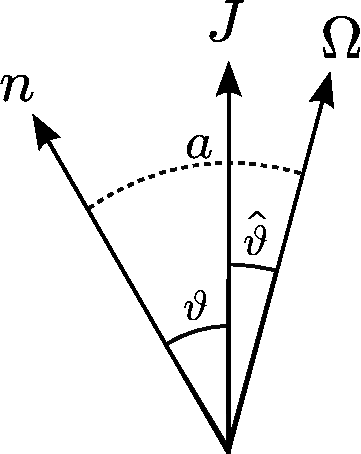
\includegraphics[width=0.2\textwidth]{ReferencePlane.pdf}
    \caption{The reference plane containing the angular momentum vector $\spin$,
    the angular momentum vector $\mathbf{J}$ and the deformation axis $\mathbf{n}$.}
    \label{fig: reference plane}
\end{figure}
In this figure, we have defined the angle between anglular momentum and $\n_a$ as
$\theta$, conventionally referred to as the \emph{wobble-angle} of
precession. We have also given $a$, the angle between the 3-axis and the
spin-vector as defined in Sec.~\ref{sec: rotating frame}.

Let us now decompose the angular velocity into the Euler angle components along
the angular momentum and deformation axis (these are the same Euler angles as defined in
Sec.~\ref{sec: euler rotation matrices})
\begin{equation}
  \omega_a = \dot{\phi}\hat{J}_a + \dot{\psi}\n_{a},
\label{eqn: decomp}
\end{equation}
where $\hat{J}_a$ is a unit vector pointing along the angular momentum. Then,
substituting this into Eqn.~\eqref{eqn: ang mom} we find that
\begin{align}
J_a = I_0 \dot{\phi} \hat{J}_a + \left(I_0 \dot{\phi} + \Delta I \omega_z\right)\n_a.
\end{align}
Comparing components, we have that
\begin{align}
|J_a| = I_0 \dot{\phi},
\end{align}
and
\begin{align}
\dot{\psi} = -\frac{\Delta I}{I_0} \omega_3.
\end{align}
To relate the angles, we can use the $\dot{\psi}$ equation in \eqref{eqn: ODEs},
giving
\begin{align}
\dot{\psi} = - \frac{\Delta I}{I_0 + \Delta I} \dot{\phi} \cos\theta
\approx -\frac{\Delta I}{I_0} \dot{\phi} = -\epsI \dot{\phi}
\label{eqn: psi phi}
\end{align}
where we have approximated assuming $\Delta I \ll I_0$ and $\theta \ll 1$ in
the last step.

We can relate both of these frequencies to the spin frequency $|\omega|$.
First, from the cosine rule we have that
\begin{align}
|\omega_a|^{2} = \dot{\phi}^{2}+\dot{\psi}^{2} - 2\dot{\phi}\dot{\psi}\cos\theta.
\end{align}
and so rearranging and neglecting terms of order $\epsI^{2}$, we have that
\begin{align}
\dot{\phi} \approx \frac{|\omega_a|}{\sqrt{1- 2\epsI\cos\theta}}.
\label{eqn: phi dot}
\end{align}
This informs us that $\dot{\psi}$ is approximately the fast spin frequency
of the star while from Eqn.~\eqref{eqn: psi phi} we see that $\dot{\phi} \ll |\omega_a|$
is a much slower frequency, the precession frequency.

From the previous section we learnt that any vector fixed in the rotating frame
can be transformed into the inertial frame by the Euler angle rotation matrix,
Eqn.~\eqref{eqn: rotation matrix}. For torque free precession $\theta$ is a
constant \citep{Landau1969}; therefore when viewed in the inertial frame, any
fixed vector in the rotating frame can be understood as undergoing two motions:
keeping $\phi$ fixed and increasing $\psi$ rotates the vector in a cone
about the $\n_{a}$ axis at frequency $\dot{\psi}$; holding
instead $\psi$ fixed and increasing $\phi$ sweeps the vector about a cone
centred around the $\hat{J}_a$ axis at frequency
$\dot{\phi}$. The motion of the fixed vector is the superposition of these two
rotations; the $\psi$ rotation is referred to as precession and happens at a
slower frequency as seen from Eqn.~\eqref{eqn: psi phi}.

We will now understand the motion of $\m$, the magnetic dipole, under torque
free precession. We will do this initially by application of the Euler angle
rotations and then we will return to this reference frame picture in
Sec.~\ref{sec: understanding the motion of m} to provide a deeper intuitive
understanding.

\subsection{Dynamics of the magnetic dipole}

Numerical solutions to Eqn.~\eqref{eqn: ODEs} allow us to calculate the motion
of any quantity in the inertial frame from which the neutron star is observed.
This can be used, for example, to calculate the motion of the spin-vector in the
rotating frame under any arbitrary torque. However, pulsar astronomers observe the pulsar
through the pulsations of EM emission. If this emission is colinear with the
dipole, then it points along the unit vector of the magnetic dipole $\m$. Therefore,
we are particular interested in the motion of $\m$ in the inertial frame.

In the rotating frame, we set $\m$ to lie at an angle $\chi$ to the $z'$ axis
with unit vector $[\sin(\chi), 0, \cos(\chi)]$ without loss of generality.
Using the inverse of Eqn.~\eqref{eqn: rotation matrix}, the Euler angles
rotation matrix, we can transform to the inertial frame; the components of the
magnetic dipole in the inertial frame are
\begin{equation}
\m =
\left[\begin{array}{c}
\cos\phi\cos\psi\sin\chi - \sin\phi \cos \theta \sin \psi \sin \chi
+ \sin \phi \sin \theta \cos \chi \\
\sin\phi\cos\psi\sin\chi + \cos\phi \cos \theta \sin \psi \sin \chi
- \cos \phi \sin \theta \cos \chi \\
\sin\theta \cos\psi \sin\chi + \cos\theta \cos \chi
\end{array}\right].
\label{eqn: m inertial}
\end{equation}•
Following the work of \citet{Jones2001} we define two angles $\Phi$ and $\Theta$
which describe the polar and azimuth of $\m$ in the inertial frame.
From Eqn.~\eqref{eqn: m inertial} the azimuthal angle is given by
\begin{equation}
    \Phi = \arctan\left(\frac{\m_{y}}{\m_{x}}\right) =
\phi - \frac{\pi}{2} + \arctan\left(\frac{1}{\cos\theta}
                       \left(\frac{\cos\psi \tan \chi}{\tan\theta -
                       \sin \psi \tan\chi }\right)\right),
\label{eqn: Phi}
\end{equation}
while the polar angle is
\begin{equation}
\Theta = \arccos(\m_{z}) = \arccos(\sin \theta \sin \psi \sin \chi + \cos \theta \cos \chi ).
\label{eqn: Theta 2}
\end{equation}

Eqn.~\eqref{eqn: Phi} and Eqn.~\eqref{eqn: Theta 2} are exact results and will
be used later on to derive physical observables such as the phase residuals.
Specifically, given a numerical solution of equations~\eqref{eqn: ODEs}, i.e.
the evolution of the spin-vector and three Euler angles, we can use these two
equations to describe the evolution of the magnetic dipole orientation in the
inertial frame which can subsequently be used to calculate the phase of
pulsations. Before we do this, we will build some feeling for the dynamics of
the magnetic dipole in the inertial frame in the torque free case.

Using our numerical solution, we simulate a star without any EM torque. The
resulting solutions for the Euler angles can then be substitued into Eqn.~\eqref{eqn: Theta 2}
to give the evolution of $\Theta$. This is done for three choices of $\theta$
and $\chi$ in Fig.~\ref{fig: polar angle variations}
\begin{figure}[htb]
\centering
  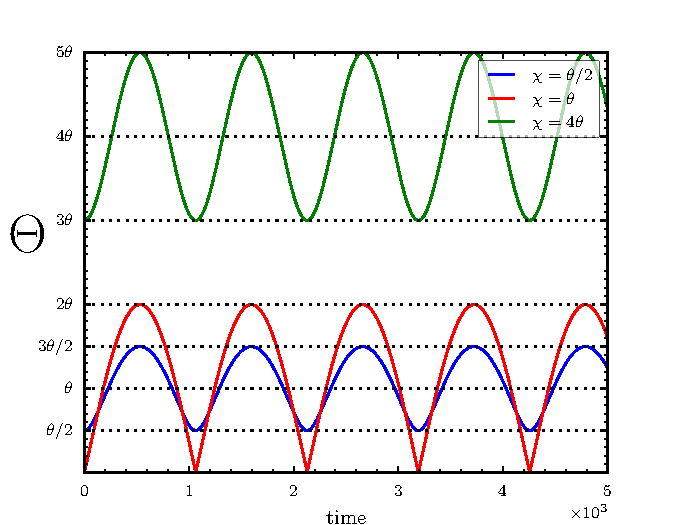
\includegraphics[width=0.7\textwidth]{polar_angle_variation_with_chi.pdf}
\caption{Variations in the polar angle of the dipole $\m$ under free precession}
\label{fig: polar angle variations}
\end{figure}
From this figure, we see that the polar angle is modulated at the precession
period, $\tauP$. In the next section we will provide a deeper understanding
of where the size of modulations comes from and the significance in the choice
of $\theta$ and $\chi$.

The spin frequency of a pulsar is the rate with which observers measure the
observed pulsations, usually we think of this as exactly the rotation frequency
$|\omega|$. However, for a precessing star the observed frequency is not given by
$|\omega|$ due to the additional motions of precession. Instead, we note that the
observer would fit a timing model to the TOAs as the pulse passes through the
plane containing them and the angular momentum vector, the phase of which is
$\Phi$. So the frequency measured would be given by the first derivative of $\Phi$:
\begin{equation}
\dot{\Phi} = \dot{\phi}
+ \frac{\sin\chi \left(
\dot{\psi} (\cos\theta\sin\chi - \sin \psi \sin \theta \cos\chi) +
\dot{\theta} \cos\psi (\cos\theta\cos\chi - \sin \psi \sin \theta \sin\chi)\right)
}{(\sin\theta \cos \chi - \cos \theta \sin \psi \sin \chi)^{2} + \cos^{2}\psi \sin^{2} \chi}.
\label{eqn: Phi_dot}
\end{equation}
This is the \emph{instantaneous electromagnetic frequency}; an observer
will measure the time averaged value of $\dot{\Phi}$ as the `spin frequency' of
the star.

In Fig.~\ref{fig: frequency variations} we plot the frequency modulations for
the three choices of $\theta$ and $\chi$ used in Fig.~\ref{fig: polar angle variations}.
Again, we see modulation at the precession period; in the following section to
will provide a deeper understanding of these modulations and the choices of
$\theta$ and $\chi$.
\begin{figure}[htb]
\centering
  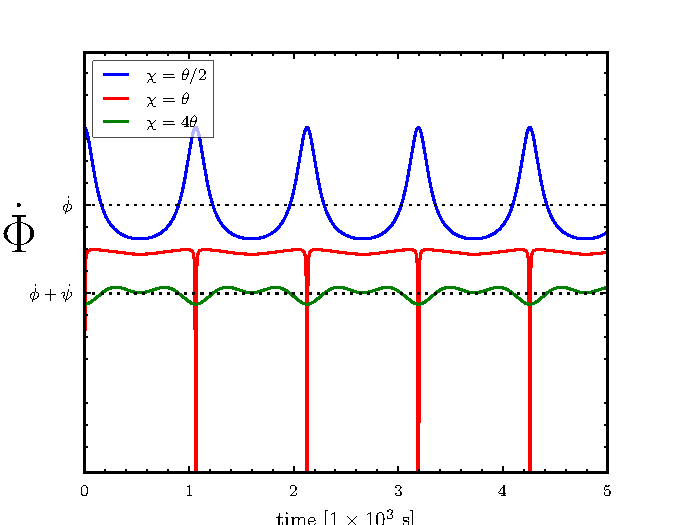
\includegraphics[width=0.7\textwidth]{frequency_variation_with_chi.pdf}
\caption{Variations in the instantaneous electromagnetic frequency for three choices
of $\chi$ and $\theta$ under free precession}
\label{fig: frequency variations}
\end{figure}


\subsection{Understanding the dynamics of the magnetic dipole}
\label{sec: understanding the motion of m}

We will now return to the reference plane picture discussed in Sec.~\ref{sec:
reference plane}. In particular, we will now provide a detailed description of
the motion of $\m$ as seen by the observer and use this to explain the
modulations seenin Fig.~\ref{fig: polar angle variations} and Fig.~\ref{fig:
frequency variations}.

From Eqn.~\eqref{eqn: decomp}, the motion of the magnetic dipole, a vector
fixed in the rotating frame, when viewed in the inertial, can be understood as
the superposition of two rotations. First, $\n_a$ is swung in a cone about the
angular momentum at $\dot{\psi} \approx |\omega$, second, superimposed on to
this $\m$ is swung in a cone about $\n_a$ at the slower precession frequency
$\dot{\psi}$. The resulting motion is best understood by considering three
choices of $\chi$ and $\theta$: $\chi < \theta$, the special case $\chi =
\theta$, and $\chi > \theta$. We we illustrate the projection of the two
cones onto the reference plane for these three choices in Fig.~\ref{fig: cones}.
\begin{figure}[ht]
\centering
	\subfloat[$\chi < \theta$]{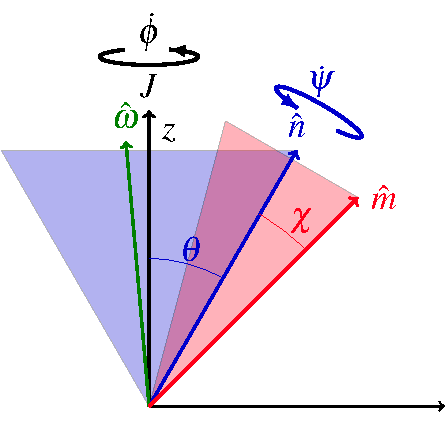
\includegraphics[width=0.33\textwidth]
    {chi_less_theta.pdf}}
	\subfloat[$\chi = \theta$]{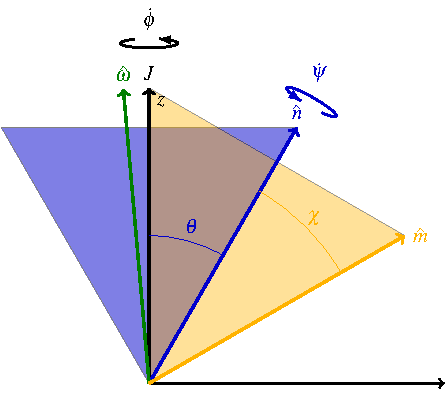
\includegraphics[width=0.33\textwidth]
    {chi_equal_theta.pdf}}
	\subfloat[$\chi > \theta$]{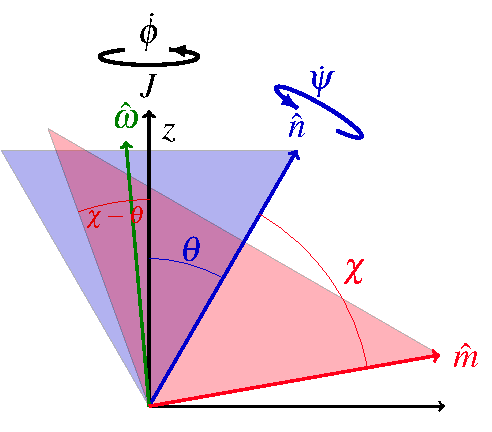
\includegraphics[width=0.33\textwidth]
    {chi_more_theta.pdf}}
\caption{Diagrams depicting 2D projections of the cones swept out by the
    different motions under torque free precession onto the reference plane.
    The yellow cone is swept out by the rotation of $\m$ about $\n_{d}$ at the
    slow precession frequency; the blue cone is swept out by the rotation of
    $\n_{d}$ about $\J$ at the fast spin frequency.}
\label{fig: cones}
\end{figure}

Since $\m$ is fixed at an angle $\chi$ to $\n_a$, it too is swung in a cone
about the angular momentum vector at $\dot{\phi}\approx |\omega|$; if EM
radiation is emitted along this axis then this motion is precisely the
pulsations which give pulsars their name.  However, $\m$ alse rotates about
$\n_a$ during a precessional cycle, but this modulation is slower by a factor
$\epsI$ compared to the spin frequency. We can then imagine the motion of $\m$
as seen by on observer as a cone, the \emph{dipole cone}, swept out by $\m$ at
the fast spin frequency; the half-angle of this cone will be exactly $\Theta$
and will be modulated at the precession period (as shown in Fig.~\ref{fig:
polar angle variations}).  The frequency with which $\m$ rotates around dipole
cone is $\dot{\Phi}$ given by Eqn.~\eqref{eqn: Phi_dot}. Let us now describe
the evolution of the dipole cone for the three cases in Fig.~\ref{fig: cones}:
\begin{itemize}
\item The $\chi < \theta$ case ($\chi = \theta/2$): the precession cone is
narrow and does not extend over the angular momentum vector. The polar angle
$\Theta$ of the dipole cone oscillates periodically between $\theta+\chi$ and
$\theta-\chi$ during a precession cycle, as shown in Fig.~\ref{fig: polar angle
variations}.  The spin frequency $\dot{\Phi}$ (see Fig.~\ref{fig: frequency
variations} has an average value of $\dot{\phi}$ and oscillates about this
value, comparing with the $\Theta$ variations demonstrates these oscillations
are locked in phase with the rotation of $\m$ in the precession cone. Recalling
that the precession cone counter rotates with respect to the spin cone, at
$\theta+\chi$ the precession cone motion acts in the opposing direction to the
spin cone, this causes a reduction in the spin frequency away from the average;
by contrast at $\theta-\chi$ the counter rotation is now in favour of the spin
frequency and as a result the spin frequency is increased above the average.

\item The $\chi = \theta$ case: in this special case the angular momentum vector sits exactly
on the side of the precession cone, this suggest at certain precessional phases $\m$ can align exactly with
the angular momentum. When this happens the spin frequency tends to zero manifesting as sharp dips in the
spin frequency; at the same time the polar angle tends to zero.

\item The $\chi > \theta$ case ($\chi = 4\theta$): The precession cone now extends over the
angular momentum vector, this means it always acts to reduce the spin
frequency; as a result the spin frequency has an average value of
$\dot{\phi} + \dot{\psi}$. The polar angle can vary between $\theta+\chi$ and
$\chi-\theta$, for $\chi$ close to $\theta$ the deviations away from the
average are large while as $\chi$ increases the deviations get smaller as
the half angle of the dipole cone increases.
\end{itemize}
We will comment on these results further by verifying them numerically in
Fig.~\ref{fig: polar angle variations} and Fig.~\ref{fig: frequency variations}.

\meta{..}
Additionally for the two cases $\chi>\theta$ and $\chi < \theta$ we have
plotted the average spin frequencies $\dot{\phi}$ and $\dot{\phi}+\dot{\psi}$
as predicted by \citet{Jones2001}. This shows the periodic modulations in all
three instances, and the instantaneous drop in spin frequency to zero in the
case of $\chi=\theta$.

\section{The effective wobble angle}
\label{sec: wobble angle}
The angle $\theta$ (see Fig.~\ref{fig: reference plane})) is referred to as the
\emph{wobble angle} since, in torque-free precession, its magnitude determines
the `amount' of precession.  In Eqn.~\eqref{eqn: psi phi}, we demonstrated that
for nearly spherical stars where $\epsI \ll 1$ and when $\theta \ll 1$ the
angles are related by
\begin{align}
\hat{\theta} \approx \epsI\theta.
\label{eqn: theta hat theta}
\end{align}
Consequently, from Fig.~\ref{fig: reference plane} we see that $a\approx
\theta$.

When including the EM torque the wobble angle
does not have the intuitive interpretation of the `amount' of precession.  In
particular, the anonalous part of the torque defined Eqn.~\eqref{eqn: torque}
can be understood to create an effective rotating frame as shown in Sec.~\ref{sec:
effective body frame}. This means that solutions exist which appear to undergo
`peristent precession' where $\theta \approx a\ne0$ such that the body remains
misaligned from the principal axes of its moment of inertia tensor. However, we
demonstrated that in fact the body has alligned with the principal axes of
it \emph{effective} moment of inertia tensor.

Let us then define a an effective wobble angle
\begin{align}
\wobbleangle = \theta - \beta.
\label{eqn: wobble angle}
\end{align}
That is, we rotate by the angle $\beta$ defined in Eqn.~\eqref{eqn: beta}. In
the limit where $\beta \rightarrow 0$ we recover the usual wobble angle referred
to by \citet{Jones2001} $\theta = \wobbleangle$, but if the effects of the
anomalous torque are important then the effective wobble angle $\wobbleangle$ will
measure the amount of precession (i.e. its magnitude determines the amplitude
of precession). This definition will be used later on when setting up solutions
which initially have a minimal amount of precession.



%\subsection{Pulse frequency and polar angle under torqued precession}
%Having a physical understanding of why $\Theta$ and $\dot{\Phi}$ evolve under
%free precession as in Fig.~\ref{fig: polar angle variations} and Fig.~\ref{fig:
%frequency variations}, we will study what happens to such a system when
%including the effects of the EM torque.
%
%In Fig.~\ref{fig: polar angle variations with torque}  we give the variations in
%the polar angle under torqued precession.The torque introduces two
%additional effects: $\dot{\Phi}$ the instantaneous electromagnetic frequency
%decays slowly, this is caused by the spin down torque and is full agreement
%with what we expect; a fast sinusoidal oscillation in $\dot{\Phi}$ on the spin
%time scale, observable as a broadening of the line, is a result of the
%anomalous torque. As for the polar angle $\Theta$ the anomalous torque causes
%slight changes in the limits of the sinusoidal variation. Both the anomalous
%torque effects can be understood by realising that this effectively adds a
%triaxiality into the moment of inertia tensor. % needs more explanation
%
%\begin{figure}[ht]
%\centering
%	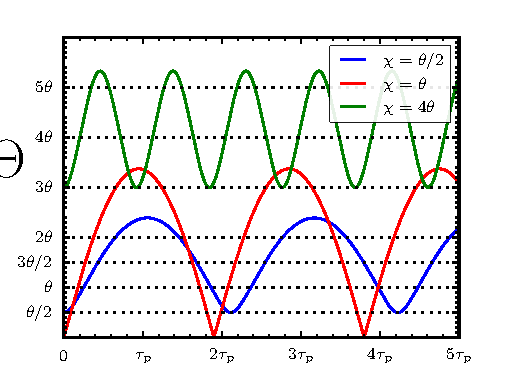
\includegraphics[width=0.7\textwidth]{polar_angle_variation_with_chi_inc_torque.pdf}
%\caption{Variations in the polar angle of the dipole $\m$ under torqued precession}
%\label{fig: polar angle variations with torque}
%\end{figure}
%
%\begin{figure}[ht]
%\centering
%	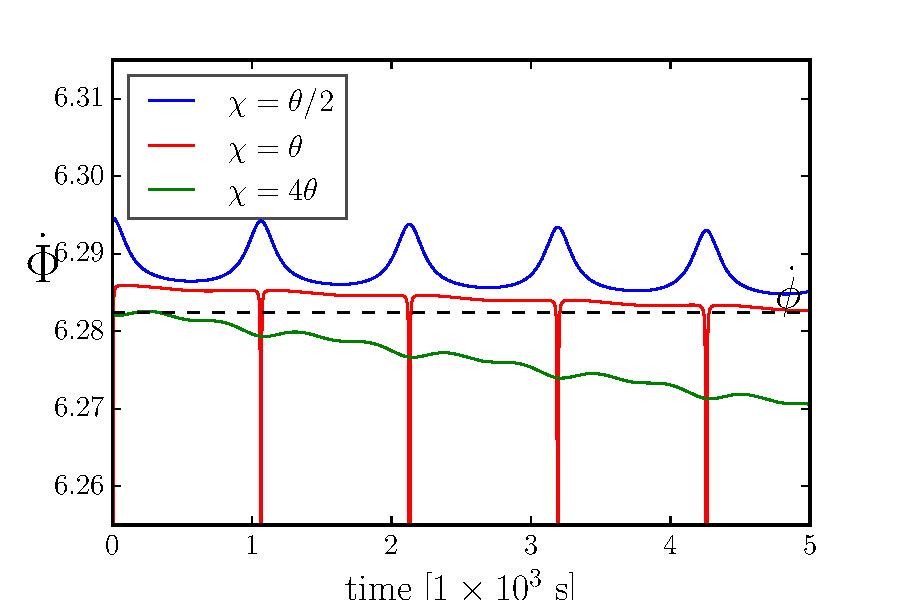
\includegraphics[width=0.7\textwidth]{frequency_variation_with_chi_inc_torque.pdf} \\
%\caption{Variations in the spin-frequency of the dipole $\m$ under torqued precession}
%\label{fig: frequency variations with torque}
%\end{figure}

\section{Physical observables: phase residuals}
\label{sec: timing residuals}

The principal observational quantify reported on for a pulsar is the timing
residual. This is the difference between the measured TOA of a pulse and a
timing model of the pulsar as discussed in Sec.~\ref{sec: pulsar timing
methods}. It is the remaining structure in the timing residual which we
often call `timing-noise' so let us now discuss how this can be calculated
from our numerical model after which we will compare this with analytic
estimates. Note that timing residuals and phase residuals are approximately
equivalent, we will discuss this once we have defined the phase residual.

The azimuthal angle $\Phi$ given in Eqn.~\eqref{eqn: Phi} gives us the phase of
the magnetic dipole. For the observer, the pulsation occurs when the dipole
passes through the plane containing the observer and the angular momentum
vector,  we can always reorient the observer such that the pulsation occurs
every time $\Phi$ is a multiple of $2\pi$. In this way, $\Phi$ is also the
phase of the observed pulsations. To generate $\Phi$ we define the stars
properties i.e. the magnetic field and initial angles, then numerically
evolve equations~\eqref{eqn: ODEs}. The resulting time series of the spin-vector
components and Euler angles are then substituted into Eqn.~\eqref{eqn: Phi} to
generate the exact phase.

Following the methods used by observers, we define our `timing model' as
a Taylor expansion to the phase about some reference time $\tref$ up to $\ddot{f}$:
\begin{equation}
    \Phifit(t; \tref, \f, \fdot, \fddot) =
    2\pi \left(\f(t - \tref) +
                          \frac{\fdot}{2!}(t-\tref)^{2} +
                          \frac{\fddot}{3!}(t-\tref)^{3}
                          \right),
\label{eqn: TR taylor expansion}
\end{equation}
with the timing properties ($f$, $\dot{f}$, $\ddot{f}$) as free parameters.
Higher order terms can be included, as discussed in Sec.~\ref{sec: timing noise
observations}, but here we truncate at $\ddot{f}$. We do not include an initial
phase since we can arbitrarily define our reference time to coincide with a
pulsation such that the initial phase is zero.  Unlike pulsar astronomers, we
do not need to worry about other corrections such as the motion of the Earth
since $\Phi$ is given in the inertial frame.

The phase residual is then the difference between the exact phase
and the fitted phase
\begin{equation}
  \Delta\Phi(t) = \Phi(t) - \Phifit(t; \tref, \phi, \f, \fdot, \fddot).
\end{equation}
We then use a least-squares fitting method to minimise the root mean squared
error of the phase residual. The fitted coefficients $\{\phi, \f, \fdot,
\fddot\}$ constitute out best-fit phase model: the best fit to the data
$\Phi(t)$ of a power law spin-down model.  It is worth noting that a residual
depends on which section of data was used in the fit.

Finally, the phase residual can also be re-scaled to give the timing residual by
calculating the residual as a fraction of a cycle then multiplying by the
period
\begin{equation}
    \Delta T = \frac{\Delta\Phi(t)}{2\pi} P.
    \label{eqn: phase to timing}
\end{equation}
Over a typical observation periods it is possible for the period to
fractionally change due to the spin-down, but the effect is negligible compared
to the other variations considered in this work. Therefore, we will report only
on phase-residuals.

In the following subsections we will compare analytic results for the phase
residuals due to precession with our numerical results found by fitting and
removing a polynomial. As shown in Sec.~\ref{sec: underting the motion of m}
the form of solution will depend on whether $\chi < \theta$ or $\chi > \theta$.
Of these two choices, \citet{Jones2001} concluded that `the wobble angle of
rapidly rotating stars are limited to small values for the finite crustal
breaking strain'; following this reasoning we will limit our stufy to the
$\chi > \theta$ case although the numerical code is capable of finding solutions
for either.

\subsection{Effect of precession on the phase residual}

The effect of free precession on phase residuals was considered by \citet{Nelson1990},
since these modulations are independent of the torque, they are referred to as
the \emph{geometric effect}. To calculate a phase residual, \citet{Jones2001}
subtracted the secular phase evolution from Eqn.~\ref{eqn: Theta 2} and,
after some manipulation found that the phase residual when $\chi > \theta$ is
given by
\begin{equation}
    \Delta\Phi_{49}(t) = -\theta \cot\chi\cos\left(\dot{\psi}t + \frac{\pi}{2}\right),
    \label{eqn: Jones 49}
\end{equation}
where the subscript here refers to the equation number of \citet{Jones2001}.
For a precessing star $\dot{\psi}$ is given by Eqn.~\eqref{eqn: psi dot} and
the initial value of the cosine argument is $\psi(t=0)=\pi/2$ as derived in
Sec.~\ref{sec: initial conditions}.

Equation \eqref{eqn: Jones 49} is calculated in the absence of any EM torque.
Nevertheless, it is still appropriate when a torque is applied provided
that the geometric effect is stronger that any other (this is discussed in
the next few sections). As such, we begin by simulating a NS with the properties
listed in table \ref{tab: PR 49}.
\begin{table}
\centering
\begin{tabular}{ccl}
\multicolumn{3}{c}{Simulation parameters} \\
\hline
$\omega_0$  &=& 10.0 rad/s\\
$B_0$  &=& ${1.0}{\times} 10^{13}$ G \\
$\chi$  &=& 50.00$^{\circ}$ \\
$a_0$ &=& 2.00$^{\circ}$ \\
$\tilde{\theta}$ &= & 2.00$^{\circ}$ \\
$\mathcal{A}_{\mathrm{EM}}$ &= & ${4.3}{\times} 10^{-6}$
\end{tabular}
\caption{Simulation parameters used for the phase residual plotted in Fig.~\ref{fig: PR 49}}
\label{tab: PR 49}
\end{table}
The resulting phase residual, in cycles, is
given in Fig.~\ref{fig: PR 49}.
\begin{figure}[htb]
\centering
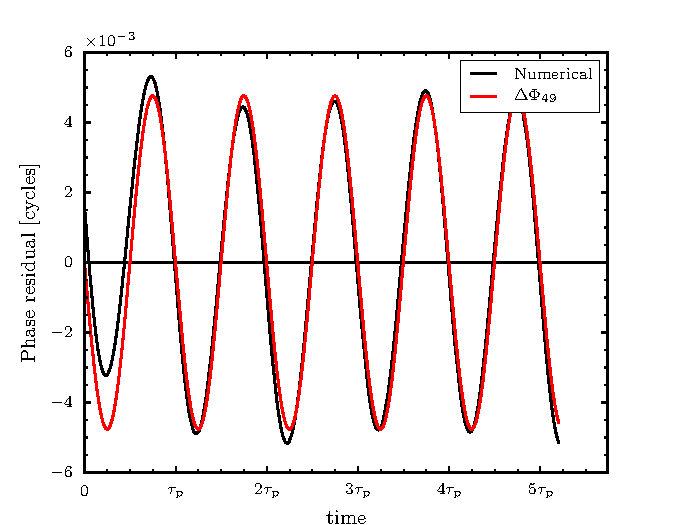
\includegraphics[width=0.8\textwidth]{49_verification}
\caption{The simulated phase residual in cycles for a simulated NS with the
properties described in Table~\ref{tab: PR 49}. We also plot the corresponding
analytic prediction of Eqn.~\eqref{eqn: Jones 49}}
\label{fig: PR 49}
\end{figure}

This figure shows strong agreement between the numerical result and the
analytic prediction of Eqn.~\eqref{eqn: Jones 49}. The numerical result does
show an what appears to be a periodic difference with a half period equal to
the data span. This is due to inaccuracies in the fitting procedure and was
verified by changing the data span and observing that the half period shifted
accordingly.


\subsection{Effect of torqued precession on the phase residual: electromagnetic amplification}
\label{sec: phase residual torqued}

The geometric effects of precession can be amplified by the EM torque \citep{Cordes1993}.
Using a simple description based on a vacuum point-dipole spin-down torque,
and calculating the departure from a non-precessing power-law spin-down,
the amplified phase residuals are given by
\begin{align}
\Delta\Phi_{63} = -\frac{1}{\pi}\left(\frac{\tau_{P}}{P}\right)
                               \left(\frac{\tau_{P}}{\tauAge}\right)
                               \cot\chi
                               \sin(\dot{\psi} t + \pi/2)
\label{eqn: Jones 63}
\end{align}
This result is derived in \citet{Jones2001} for the magnitude of modulations, here
we keep the exact time evolution behaviour intact. Notably, we can write the
magnitude of modulations in term of Eqn.~\eqref{eqn: Jones 49} as
\begin{equation}
    |\Delta\Phi_{63}| = \frac{1}{\pi}\left(\frac{\tau_{P}}{P}\right)
    \left(\frac{\tau_{P}}{\tauAge}\right)
                                    |\Delta\Phi_{49}|
\label{eqn: Jones 63 mag}
\end{equation}
The two ratios of time-scales define an `amplification factor'
\begin{equation}
    \mathcal{A}_{\mathrm{EM}} = \left(\frac{\tau_{P}}{P}\right)
                                \left(\frac{\tau_{P}}{\tauAge}\right).
\label{eqn: EM amplification}
\end{equation}
The amplification, as first noted by \citet{Cordes1993}, will increases the
magnitude of phase residuals for young pulsars with short periods. It is worth
noting however, that there is a relative phase difference between
Eqn.~\eqref{eqn: Jones 49} and Eqn.~\ref{eqn: Jones 63}.

To verify this amplification, we simulate a star using the properties in
Table~\ref{tab: PR 63} for which the amplification factor is greater than
unity.
\begin{table}
\centering
\begin{tabular}{ccl}
\multicolumn{3}{c}{Simulation parameters} \\
\hline
$\omega_0$  &=& $10^{4}$ rad/s\\
$B_0$  &=& $ 10^{14}$ G \\
$\chi$  &=& 50$^{\circ}$ \\
$a_0$ &=& 2$^{\circ}$ \\
$\mathcal{A}_{\mathrm{EM}}$ &= & $43$
\end{tabular}

\caption{Simulation parameters used for the phase residual plotted in Fig.~\ref{fig: PR 63}}
\label{tab: PR 63}
\end{table}
The resulting phase
residual is plotted in Fig.~\ref{fig: PR 63} along with the predictions of
Eqn.~\eqref{eqn: Jones 63} and Eqn.~\eqref{eqn: Jones 49}. This clearly demonstrates
that the amplified residuals agree with the results calculated
numerically.
The resulting phase residual, in cycles, is
given in Fig.~\ref{fig: PR 49}.
\begin{figure}[htb]
\centering
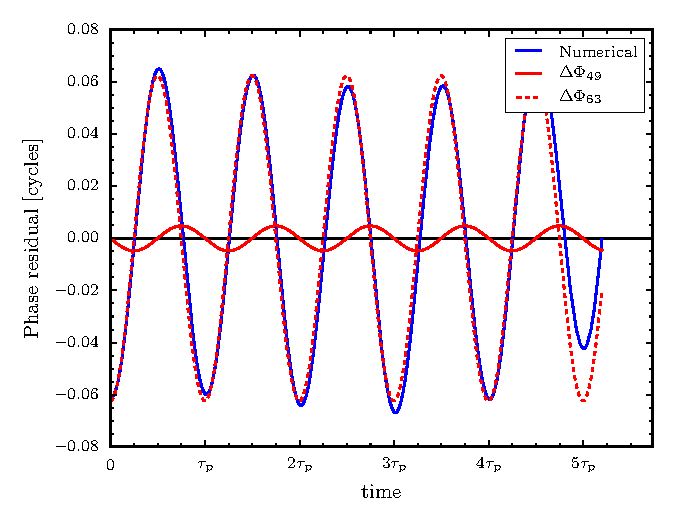
\includegraphics[width=0.8\textwidth]{63_verification}
\caption{The simulated phase residual in cycles for a simulated NS with the
properties described in Table~\ref{tab: PR 63}. We also plot the corresponding
analytic prediction of Eqn.~\eqref{eqn: Jones 49} and Eqn.~\eqref{eqn: Jones 63}}
\label{fig: PR 49}
\end{figure}

\section{Physical observables: spin-down rate}

The derivatives of the phase (the frequency and spin-down rate) display similar
long term departures to their secular evolutions: periodic modulations which
can be amplified by the EM torque.  We have already, in Fig.~\ref{fig:
frequency variations}, investigated the modulations of the frequency due to
free precession. However, long term modulations of the frequency (on top of the
usual secular spin-down), are not reported in the literature. Therefore, the
second physical observable that we will consider is the \emph{spin-down rate}.

PSR~B1828-11 is a normal radio pulsar which displays strong periodic modulation
in its spin-down rate. This has been modelled analytically by several authors
\citep{Stairs2000, Jones2001, Link2001, Akgun2006} who all found that the timing
residuals and spin-down rate modulations were consistent with EM-dominated
precession. We can confirm this by noting that the inferred precession period for this
pulsar is $\tauP \approx 500$~days, the period is $P\approx0.405$~s, and
the spin-down age is $\tauAge = P/\dot{P} \approx 2.1 \times10^{5}$~yrs (values
taken from the ATNF catalouge \citet{ATNF}), therefore
\begin{align}
\Aem \approx 682.
\end{align}
In this section we will derive an analytic model appropriate for this pulsar
which will be used in Chapter.~\ref{sec: testing models} in a model comparison
for PSR~B1828-11. Then, we will compare this analytic model with a spin-down
rate calculated numerically and understand the various regimes. We will not
consider the geometrically dominated spin-down rate modulations, further
details on that subject can be found in \citet{Jones2001}.

To calculate spin-down rates numerically, we could calculate the pulse phase
(Eqn.~\eqref{eqn: Phi 2}) and then numerically differentiate to get
$\ddot{\Phi}$. However, when studying the long-term modulations in the spin-down
rate observers (see for example \citet{Lyne2010, Perera2015}) use what we will
refer to as the \emph{observer-method}: a second order Taylor expansions is
fitted to short sections of data of length $T$ and the resulting coefficient
$\ddot{\nu}$ is recorded at the mid-point of the section of data; repeating
this process every $\sim T/4$ in a `sliding-window' builds a picture of how the
spin-down varies with time.  We will mimic this data collection process by
fitting Taylor expansions to short sections of the simulated phase $\Phi$. This
has the benifit that we include any potential perculiarities of the data
collection mechanism in our simulation.  We choose $T$ such that it is a
fraction of the precession period over which we expect quantities to be
modulated. This is consistent with the observers-method where $T$ is chosen in
order to resolve the observed modulations.

\subsection{Derivation of the precession spin-down rate}
\label{sec: derivation of spin-down rate}
Let us known derive the spin-down rate for a precessing pulsar under a
vacuum point-dipole spin-down torque. Similar derivations have been found by
\citet{Link2001} and \citet{Jones2001}, this is given primarily as a complete
derivation of the spin-down rate used in Chapter.~\ref{sec: testing models}
and published in \citet{Ashton2016}.

From the definition of the vacuum point-dipole spin-down torque we have that,
\begin{align}
\ddot{\Phi} = -k \dot{\Phi}^{n} \sin^{2}\Theta,
\label{eqn: EM DE}
\end{align}
where $k$ is a positive constant. From \citet{Jones2001}, we also have
\begin{align}
\cos\Theta = \sin\theta \sin \psi \sin \chi + \cos\theta \cos\chi.
\end{align}
Rearranging and expanding about $\theta = 0$, we find
\begin{align}
\sin^{2}\Theta & =
\left[
\sin^{2}\chi + \theta^{2}\left(\cos^{2}\chi - \frac{\sin^{2}\chi}{2}\right)
\right]
- 2\theta \sin\chi\cos\chi \sin\psi
 + \frac{1}{2}\theta^{2}\sin^{2}\chi\cos(2\psi),
\label{eqn: sin 2 Theta}
\end{align}
where the first term, in square brackets, is a constant while the second two
terms provide the first and second harmonic modulations in $\psi(t)$.

In order to find approximate solutions to Eqn.~\eqref{eqn: EM DE}, we begin by
defining the time-averaged (constant) value of $\sin^{2}\Theta$ as
\begin{align}
\sin^{2}\Theta_0 =
\sin^{2}\chi + \theta^{2}\left(\cos^{2}\chi - \frac{\sin^{2}\chi}{2}\right),
\label{eqn: sin2Theta0}
\end{align}
then solving Eqn.~\eqref{eqn: EM DE} with this constant value we get
\begin{align}
\dot{\Phi}(t) = \left(\frac{1}{\dot{\Phi}_0^{(n-1)}}
                      + (n-1)k\sin^{2}\Theta_0 t + \right)^{\frac{-1}{n-1}},
\label{eqn: zeroth order soln}
\end{align}
where $\dot{\Phi}_0 = \dot{\Phi}(0)$. Now we define the spin-down time-scale as
\begin{align}
\tauAge = \frac{|\dot{\Phi}_0|}{|\ddot{\Phi}_0|}
\approx \frac{1}{k|\dot{\Phi}_0|^{(n-1)} \sin^{2}\Theta_0}.
\end{align}
Rearranging gives
\begin{align}
k = \frac{1}{\tauAge \dot{|\Phi}_0|^{(n-1)} \sin^{2}\Theta_0}.
\end{align}
Then Eqn.~\eqref{eqn: zeroth order soln}, our zeroth-order solution to the
spin-down (under a constant $\Theta$), can be written as
\begin{align}
\dot{\Phi}(t) = \dot{\Phi}_0\left(1 + (n-1)\frac{t}{\tauAge}\right)^{\frac{-1}{n-1}}.
\label{eqn: zeroth order soln complete}
\end{align}

Now, we substiture Eqn.~\eqref{eqn: zeroth order soln complete} back into
Eqn.~\eqref{eqn: EM DE} along with the expanded, but complete variation in
$\sin^{2}\Theta$, given by Eqn.~\eqref{eqn: sin 2 Theta}.
\begin{align}
\begin{split}
\ddot{\Phi}(t)  = {} & \frac{-1}{\tauAge |\dot{\Phi}_0|^{(n-1)} \sin^{2}\Theta_0}
\dot{\Phi}_0^n\left(1 + (n-1)\frac{t}{\tauAge}\right)^{\frac{-n}{1-n}} \\
& \times \left(\sin^{2}\Theta_0
- 2\theta \sin\chi\cos\chi \sin\psi
 + \frac{1}{2}\theta^{2}\sin^{2}\chi\cos(2\psi).
\right)
\end{split}
\end{align}
In principle, this is complete and constitutes an approximation of the spin-down
under precession.
To simplify this expression, we expand the second bracket with $t/\tauAge\ll1$, then
\begin{align}
\begin{split}
\ddot{\Phi}(t) = {} & \frac{1}{\tauAge} \dot{\Phi}_0
\left(-1 + n\frac{t}{\tauAge} +
\frac{1}{\sin^{2}\Theta_0}\left(
2\theta \sin\chi\cos\chi \sin\psi
- \frac{1}{2}\theta^{2}\sin^{2}\chi\cos(2\psi)
\right)\right) \\
& +
\mathcal{O}\left(\left(\frac{t}{\tauAge}\right)^{2},
                 \theta\left(\frac{t}{\tauAge}\right)\right)
\end{split}
\end{align}
Next we expand $1/\sin^{2}\Theta_0$, from Eqn.~\eqref{eqn: sin2Theta0}, in $\theta$:
\begin{align}
\left(\sin^{2}\chi + \theta^{2}\left(\cos^{2}\chi - \frac{\sin^{2}\chi}{2}\right)\right)^{-1}
\approx
\frac{1}{\sin^{2}\chi} + \mathcal{O}(\theta^{2}).
\end{align}
Note that we only to expand to this order since this term is multiplied by a
factor of $\theta$ and we are neglecting $\mathcal{O}(\theta^{3})$ terms.
Then simpifying we have
\begin{align}
\ddot{\Phi}(t) = \frac{1}{\tauAge} \dot{\Phi}_0
\left(-1 + n \frac{t}{\tauAge} +
\left( 2\theta \cot\chi \sin\psi
- \frac{1}{2}\theta^{2}\cos(2\psi)
\right)\right).
\end{align}
Finally, converting to spin-frequencies and periods
\begin{align}
\dot{\nu}(t) = \frac{1}{P\tauAge}
\left(-1 + n \frac{t}{\tauAge} +
2\theta \cot\chi \sin\psi
- \frac{1}{2}\theta^{2}\cos(2\psi)
\right)
\label{eqn: spin-down rate}
\end{align}

The $\mathcal{O}(\theta)$ modulation term in this expression can be calculated
by differentiating Eqn.~\eqref{eqn: Jones 63} twice; this reflects that this
spin-down rate prediction includes the amplification of the EM torque. When
$\Aem < 1$, this is prediction is not suitable since the geometric variations
(derivatives of Eqn.~\eqref{eqn: Jones 49}) will dominate. We will not consider
the geometric dominated spin-down rates in this work, although our simulation
code was tested against known analytic results and found to agree.

\subsection{Modulation of the spin-down rate}
To verify that Eqn.~\eqref{eqn: spin-down rate} accurately models the spin-down
rate evolution of precessing pulsars in an EM amplification regime, we simulate
a star with the properties given in Table~\ref{tab: spin-down rate normal}.
Most significantly, $\Aem \ll 1$, which ensures that the EM torque amplifies
the spin-down rate modulations. We use an initial spin frequency $\omega_0$
much larger than typical values, this is to allow the numerical solutions to
evolve with reasonable computational power; for more physical values the
solutions are qualitatively unchanged.
\begin{table}[htb]
\centering
\begin{tabular}{ccl}
\multicolumn{3}{c}{Simulation parameters} \\
\hline
$\omega_0$  &=& 1550.0 rad/s\\
$B_0$  &=& ${1.6}\times 10^{14}$ G \\
$\chi$  &=& 50.0$^{\circ}$ \\
$a_0$ &=& 4.0$^{\circ}$ \\
$\tilde{\theta}$ &= & 4.0$^{\circ}$ \\
$\mathcal{A}_{\mathrm{EM}}$ &= & $41.0$
\end{tabular}

\caption{Simulation parameters for the spin-down rate plotted in Fig.~\ref{fig:
spin-down rate normal}}
\label{tab: spin-down rate normal}
\end{table}

The numerical spin-down rate variations, calculated using th observer-method
are plotted along with the analytic predictions of Eqn.\eqref{eqn: spin-down rate}
in Fig.~\ref{fig: spin-down rate normal}.
\begin{figure}[htb]
\centering
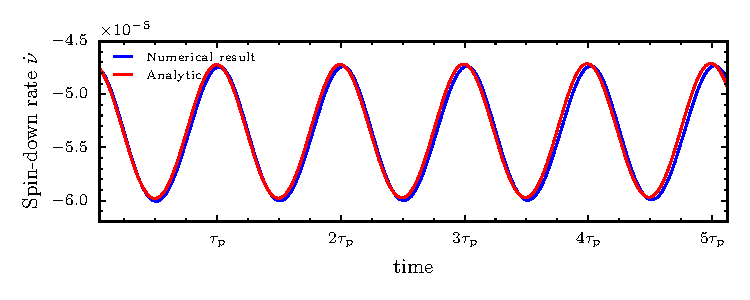
\includegraphics[]{SpindownRate_normal}
\caption{Spin-down rate for simulation parameters listed in Table~\ref{tab:
spin-down rate normal} compared against the corresponding analytic prediction
of Eqn.\eqref{eqn: spin-down rate} }
\label{fig: spin-down rate normal}
\end{figure}
This figure demonstrates good agreement: small variations result from the
application of the observer-method, most notably the numerical results under
and over estimates the minimum and maximums due to the time averaging.

\subsection{Modulation of the spin-down rate: PSR~B1828-11} While
Fig.~\ref{fig: spin-down rate normal} captures the essential features of
spin-down rate modulation amplified by an EM torque it lacks one essential
feature. Most notably this is the `double-peaked' spin-down rate which is
observed in PSR~B1828-11 \citep{Lyne2010} (see also Chapter.~\ref{sec: testing
models}) and PSR~0919+06 \citep{Perera2015}.

This double-peak is a prediction of the precession model when $\theta \ll 1$
and $\chi$ is close to $\pi/2$. This can be seen directly from the
$\mathcal{O}(\theta^{2})$ term in Eqn.~\eqref{eqn: spin-down rate}: when $\chi
\sim \pi/2$, we get a second harmonic at $\tauP/2$. To illustrate this we will
repeat the simulation of the previous section, but set $\chi=88^{\circ}$; the
full set of simulation parameters are listed in Table~\ref{tab: spin-down rate
orthog}
\begin{table}[htb]
\centering
\begin{tabular}{ccl}
\multicolumn{3}{c}{Simulation parameters} \\
\hline
$\omega_0$  &=& $10^{4}$ rad/s\\
$B_0$  &=& $10^{14}$ G \\
$\chi$  &=& 85$^{\circ}$ \\
$a_0$ &=& 10$^{\circ}$ \\
$\mathcal{A}_{\mathrm{EM}}$ &= & $75$
\end{tabular}

\caption{Simulation parameters for the spin-down rate plotted in Fig.~\ref{fig:
spin-down rate orthog}}
\label{tab: spin-down rate orthog}
\end{table}
The spin-down rate for this `almost orthogonal' dipole simulation is plotted
in the top panel of Fig.~\ref{fig: spin-down rate orthog} and demonstrates the
distinctive double peak.
\begin{figure}[htb]
\centering
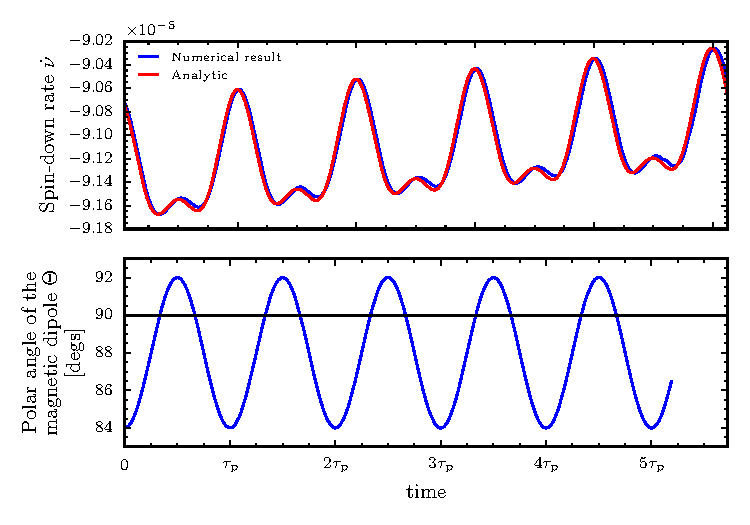
\includegraphics[]{SpindownRate_orthog}
\caption{Top panel: spin-down rate for simulation parameters listed in Table~\ref{tab:
spin-down rate normal} compared against the corresponding analytic prediction
of Eqn.\eqref{eqn: spin-down rate}. Bottom panel: the variation in the polar
angle of the magnetic dipole, $\Theta$, for the simulation.}
\label{fig: spin-down rate orthog}
\end{figure}
We can understand this feature by recalling that the dipole-cone (introduced in
Sec.~\ref{sec: understanding the motion of m}) is the
the cone swept out by $\m$ at the fast spin frequency; the half-angle this cone
makes with the angular momentum vector is $\Theta$ (see Eqn.~\eqref{eqn: Theta 2}).
In the lower panel of Fig.~\ref{fig: spin-down rate orthog} we plot this polar
angle for the same simulation. Notably the occurance of the double-peak in the
spin-down rate coincides with times when $\Theta > 90^{\circ}$. What we are seeing
is the magnetic dipole entering the lower hemisphere of the star. By considering
the form of the \citet{Deutsch1955} torque, we see that it is maximum when
the dipole perpindicular to the spin-vector. As such, when $\Theta \approx 90^{\circ}$
we have a maximum in the absoluate spin-down rate, as $\Theta$ gets larger than
this the absolute value decreases again causing the distinctive double-peak
in the spin-down rate.


\section{Physical observables: the shape of pulsation}

So far we have considered physical observables which are calculable from the
timing properties of the star: the rate at which pulses occur. However, pulsar
astronomers also discuss the shape of the pulsation by averaging over many
pulses to form an integrated pulse profile. This pulse profile is sensitive to
both the geometry of the beam itself, and the angle made between the beam and
the observer.  In this section we will discuss the variations in this angle due
to precession and then discuss the variations in the observed pulse assuming a

Let us define an observer fixed in the inertial frame such that they
maintain a constant angle $\iota$ with the angular momentum of the star $\J$.
For this observer, a pulse can be defined as the moment the dipole cuts through
the plane containing them and the angular momentum vector. At this moment, the
angle between them and the dipole will be determined by both $\iota \in [0, \pi]$ and
$\Theta \in [0, \pi]$. In particular, the angle between the observer and the beam
is given by
\begin{equation}
\Delta\Theta = \Theta - \iota
\label{eqn: delta Theta}
\end{equation}

Since $\iota$ is fixed, variations in $\Delta\Theta$ come solely from variations
in the polar angle $\Theta$. We studied these variations in Fig.~\ref{fig:
polar angle variations} and found that the $\Theta$ has an average value of the
larger of $\theta$ or $\chi$, then oscillates about this on the precession period
with a magnitude of $\theta$ or $\chi$, whichever is smaller.

\subsection{Variations in the pulse intensity}

The intensity of radiation received by an observer will depend on the
orientation of the magnetic dipole with respect to the observer and the beam
geometry. It may presumably be maximal when pointing directly at the observer
and fall off as the angle between the two grows. For each rotation of the star,
the intensity will peak when the beam cuts the plane containing the observer
and the angular momentum vector; at this instance the angle between the
observer and the beam is given by Eqn.~\eqref{eqn: delta Theta}. If the star is
precessing, then the periodic pulses of intensity due to the azimuthal rotation
of the star will be modulated by the slower variations in $\Theta$ seen in
Fig.~\ref{fig: polar angle variations}.

To model this we take an observer's with azimuth and polar angle $(\PhiO, \iota)$ and then
assume the beam geometry follows Gaussian profile with a single conal emission.
This could later be adapted to include a coral emission.  For such a model of
the beam geometry, the intensity of pulsations will vary with the angular
separation of the vector from the centre of the star to the observer and the
magnetic dipole vector. By considering the intersection of these vectors with
the unit sphere, the angular separation can be shown to be
\begin{equation}
\Delta\sigma = \cos^{-1}\left(\sin(\Theta)\sin(\iota) +
                             \cos(\Theta)\cos(\iota)\cos(\Phi - \PhiO)\right)
\label{eqn: angular sep inv cos}
\end{equation}
Then, taking a Gaussian beam geometry, the intensity of the pulse will be given by
\begin{equation}
A(\Theta, \Phi, \iota, \PhiO, \sigmaB) =
A_{0} \exp\left(-\frac{\Delta\sigma^{2}(\Theta, \Phi, \iota, \PhiO)}{2\sigmaB^{2}}\right)
\label{eqn: gaussian beam intensity}
\end{equation}
where $A_{0}$ is some constant amplitude, $\sigmaB$ is a measure of the
angular beam width.

Given a value for $A_0$ and $\sigmaB$, we can use a numerical solution to the
governing ODEs to simulate this pulse intensity exactly This is done in
Fig.~\ref{fig: intensity variation} for a system where the variations in
$\Theta$ occur on a time scale not much longer than the pulse period. This
nonphysical simulation is intended to show the modulation of the individual
pulsations due to precession.
\begin{figure}[htb]
\centering
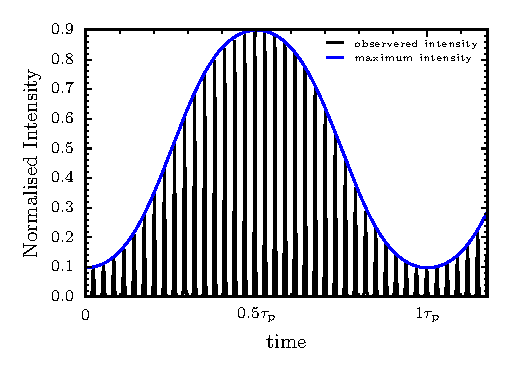
\includegraphics[width=.7\textwidth]{intensity_variation}
\caption{Amplitude variation using a 2D Gaussian emission.}
\label{fig: intensity variation}
\end{figure}
We can also predict the maximum pulse intensity at any given instance by setting
$\Phi=\PhiO$, then simplifying we find that
\begin{align}
A_{\mathrm{max}}(\Theta, \Phi, \iota, \sigmaB) =
A_{0}\exp\left(\frac{-(\Theta-\iota)^{2}}{2\sigmaB^{2}}\right),
\label{eqn: A max}
\end{align}
this is also shown in Fig.~\ref{fig: intensity variation}.

\subsection{Variations in the beam-width}
It is unlikely that the absolute variations in intensity seen in Fig.~\ref{fig:
intensity variation} will ever be unambiguously visible in nature. This is
because in real observations the intensity will also be
subject to variations in the
amount of dispersion from the interstellar medium. Therefore, pulsar astronomers
do not typically report on intensities themselves, but characterise the pulsation
by their beam-width. This is the width of the pulse at some percentage $p$ of
the observed maximum intensity. Note that this is not the maximum intensity that
the beam produces, $A_0$, but the maximum at that instant in time which is
given by Eqn.~\eqref{eqn: A max}

To model the beam-width we first note that in Eqn.~\eqref{eqn: gaussian beam intensity},
$\Theta$ varies on the slow precession timescale, while $\Phi$ varies on the
rapid spin timescale: we are looking to measure the variations with respect to
the slow precession timescale.  The pulse width is measured by the time spent
above a percentage $p$ of the maximum pulse amplitude, this can be defined as
\begin{align}
A(\Phi, \Theta, \ThetaO, \PhiO, \sigmaB) > A_{\textrm{max}} \frac{p}{100}.
\end{align}
Substituting in Eqn.~\eqref{eqn: gaussian beam intensity} and Eqn.~\eqref{eqn: A max}
then rearranging yields
\begin{equation}
\cos(\Phi - \PhiO) < \frac{
\cos\left(
\sqrt{-2\sigmaB^{2} \ln\left[\frac{p}{100}\frac{A_\textrm{max}}{A_0}\right]}\right) - \sin(\Theta)\sin(\Theta)}
                          {\cos(\Theta)\cos(\ThetaO)}
\label{eqn: 6737}
\end{equation}
where we note that $A_\textrm{max}$ is not a constant, but will evolve with the
polar angle $\Theta$ as given by Eqn.~\eqref{eqn: Theta 2}.

Let's consider a single rotation with the magnetic dipole starting and ending in
the antipodal point to the observer's position. During this rotation, $\Phi -
\PhiO$ increase between $-\pi$ and $\pi$, and so the left hand side of the
inequality is a simple cosine function as illustrated in Fig.~\ref{fig:
CosineIllustration}.  Since we expect $\Theta$ to vary slowly compared to the
rotation period we can, over a single pulsation, think of $\Theta$ as a
constant; then the whole right hand side of inequality~\eqref{eqn: 6737} is a
constant. In Fig.~\ref{fig: CosineIllustration} we illustrate this constant
along with the evolution of the left hand side: the fraction of the rotation
for which the cosine is less than the constant, i.e. inequality~\eqref{eqn: 6737}
is satisfied, defines the beam-width.
\begin{figure}[ht]
\centering
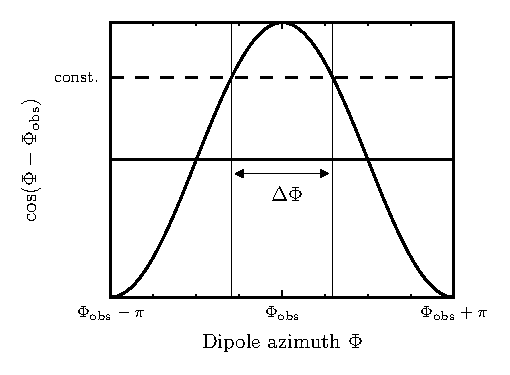
\includegraphics[width=.5\textwidth]{CosineIllustration.pdf}
\caption{Illustration of the inequality in equation \eqref{eqn: 6737} the constant
         value represents the right hand side of this equation. The
         width $\Delta\Phi$ indicates the angular period during which inequality
         is satisfied.}
\label{fig: CosineIllustration}
\end{figure}

We can calculate the beam width by first calculating the angular width $\Delta\Phi$
when the inequality is not satisfied:
\begin{equation}
    \Delta\Phi = 2\cos^{-1}\left(
                \frac{\cos\left(\sqrt{2\sigmaB^{2} \ln(f)}\right) - \sin(\Theta)\sin(\Theta)}
                          {\cos(\Theta)\cos(\ThetaO)}
                      \right).
\end{equation}
Then the angular fraction at which the inequality \emph{is} satisfied is given by
$2\pi - \Delta\Phi$. To convert this into the beam-width reported by pulsar
astronomers we multiply by the pulse period
\begin{align}
    W_{p} & = P \frac{2\pi - \Delta\Phi}{2\pi}\\
          & = \frac{1}{\pi \dot{\Phi}}\left(1 -
               \cos^{-1}\left(
                   \frac{\cos\left(\sqrt{2\sigmaB^{2} \ln(\frac{100}{p})}\right) - \sin(\Theta)\sin(\Theta)}
                          {\cos(\Theta)\cos(\ThetaO)}
                      \right)
                  \right)
\label{eqn: Wp}
\end{align}
where $P$ is the spin period which we have then written in terms of the spin
frequency and $p$ is the percentage of beam width.

\begin{table}[htb]
\centering
\begin{tabular}{ccl}
\multicolumn{3}{c}{Simulation parameters} \\
\hline
$\omega_0$  &=& 1.0 rad/s\\
$B_0$  &=& $0$ G \\
$\chi$  &=& 80.0$^{\circ}$ \\
$a_0$ &=& 6.0$^{\circ}$ \\
$\tilde{\theta}$ &= & 6.0$^{\circ}$ \\
$\mathcal{A}_{\mathrm{EM}}$ &= & $0$
\end{tabular}

\caption{Simulation parameters for the beam-width modulations plotted in
Fig.~\ref{fig: Pulse width modulation}.}
\label{tab: pulse width modulation}
\end{table}
To demonstrate an example of the beam-width modulation, in Fig.~\ref{fig: Pulse width
modulation} we plot $\Theta$ calculated from a numerical simulation with
simulation parameter listed in Table~\ref{tab: pulse width modulation} and
$W_{10}$ as calculated from Eqn.~\eqref{eqn: Wp} with $\iota=6^{\circ}$.
\begin{figure}[ht]
\centering
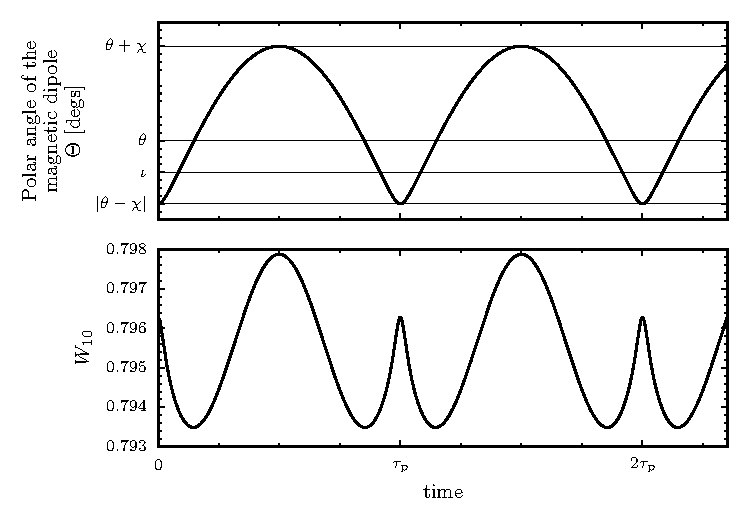
\includegraphics[]{Pulse_width_modulation.pdf}
\caption{Simulation results for the polar angle $\Theta$ and $W_{10}$, a
measure of the observed beam-width as calculated from Eqn.~\eqref{eqn: Wp}.
The simulation parameters for this are listed in Table~\ref{tab: pulse width modulation}
and we additionally set $\iota=6^{\circ}$ when calculating $W_{10}$.}
\label{fig: Pulse width modulation}
\end{figure}
This shows that there is periodic modulation of the beam-width, with an
interesting two-peak structure. This structure can be understood by realising
that the polar angle of the dipole $\Theta$ `passes over' the observer such
that for some of the precessional phase the observer sees the beam from below,
and other from above. This leads to the two-peaked structure due to the
symmetry of the emission geometry. This is a special case which depends on
the choices of $\theta, \chi$, and $\iota$: more generally the beam-width has
a single period occilatory behavior.


\section{Application: switching and precession}

Recently, some workers in the field \citep{Lyne2010, Perera2015} are suggesting
that quasi-periodic structure observed in pulsar timing residuals is a result
of magnetospheric torque-switching events as described in Sec.~\ref{sec: two
state switching}. In such models, the spin-down periodically switches between
two distinct values and these changes correlate with changes in the beam-width.
These models however are lacking a key feature: the clock which provides the
periodicity. It has been suggested \citep{Jones2012} that it may in fact be
precession which provides this clock. Ultimately, the numerical model developed
in this section could study this effect, for example by implementing a hybrid
model in which propensity for a magnetospheric switch to occur is related to
the angle $\Theta$. In this way, the observed switching would undergo
stochastic resonance as suggested by \citet{Cordes2013} and discussed in Appendix~\ref{app:
stochastic}.

In this section we will present preliminary results on a simplified hybrid model
in which we consider single switching events. We will not connect the switching
to precession, but simply consider a single switch in the torque at some time
$t_{\mathrm{switch}}$; for the time being we set this to be half the
observation period, such that $t_{\mathrm{switch}} = \To/2$.

In the EM dipole spin-down model, the torque has two distinct components: the
regular spin-down component and the anomalous component. This latter term
does not contribute to the spin-down, but as discussed in Sec.~\ref{sec: effective
body frame} will modify the axis of precession. Magnetospheric switching models
are based on evidence that the spin-down rate is switching, therefore the torque
switching must occur in the spin-down component. However, it is unclear if it would
also occur in the anomalous component, to answer this would need a detail model
of each how the magnetosphere reconfigures during a switching. We will not do
this here, but instead investigate a simple phenomenological switching in which we
modify Eqn.~\eqref{eqn: torque} as follows
\newcommand{\Ss}{S_{\mathrm{S}}}
\newcommand{\Sa}{S_{\mathrm{A}}}

\begin{equation}
\mathbf{T} = (1 - \Ss H(t-t_{\mathrm{switch}})) \mathbf{T}_{\mathrm{S}}+
                 (1 - \Sa H(t-t_{\mathrm{switch}})) \mathbf{T}_{\mathrm{A}}
\label{eqn: single switch torque}
\end{equation}
where the subscripts label the spin-down and anomalous components, $S$ is the
strength of switching, and $H(t)$ is the Heaviside step function. In this model
we can control which components are switched by choosing $\Ss$ and $\Sa$
appropriately.

In our model the strength of the EM torque is parameterised
by $\epsA$, related to the surface magnetic field strength by
\begin{align}
    \epsA = \frac{R^{5}}{4I_{0} c^{2}} B_{0}^{2}.
\end{align}
Rearranging Eqn.~\eqref{eqn: surface magnetic field} we can then write the
spin-down rate as
\begin{align}
    \dot{\omega}_{0} & = -\frac{B_{0}^{2}R^{6} \sin^{2}(\alpha) \omega_{0}^{3}}{6 I_{0} c^{3}} \\
    & = - \frac{2 R \epsA \sin^{2}(\alpha) \omega_{0}^{3}}{3 c},
\end{align}
where $\alpha$ is the angle between the spin-vector and magnetic dipole. Since
we expect these to be misaligned in order to observe pulsations, we can take
$\sin^{2}\alpha \approx 1$, then our spin-down rate is approximately
\begin{equation}
    \dot{\nu} = - \frac{R\omega_{0}^{3}}{3\pi c}\epsA.
    \label{eqn: spin-down of epsA}
\end{equation}

From this we can equate the switching in the spin-down rate $\Ss$ directly to
that measured from pulsar observations. That is, from Eqn.~\eqref{eqn: single switch torque}
we have that
\begin{equation}
    \epsA \rightarrow \epsA' = (1-\Ss)\epsA.
\label{eqn: epsA switch}
\end{equation}
during a switching, then the spin-down rate also changes as
\begin{equation}
    \dot{\nu} \rightarrow \dot{\nu}' = (1-\Ss)\dot{\nu}.
\label{eqn: nudot switch}
\end{equation}
during a switching event.


\subsubsection{Minimal precession initial state}
In the following section we will investigate the effects of a single switch, but
we first need to define a `minimal precession' initial state to which the
switch is applied so that we understand the behaviour without the switch.

Precession will not occur when the spin vector is aligned with the axis about
which it rotates. The angle between these two we have defined as the wobble
angle.  For minimal precession we should therefore set this wobble angle to
zero. In all simulations, we consider a biaxial body with the full torque given
by \eqref{eqn: single switch torque}. From our previous discussion on the
wobble angle we can minimise the precession initially by setting the initial polar angle
of the spin vector in the rotating frame to lie along the effective body-frame
axis. In the presence of the anomalous torque this is done with
\begin{equation}
a_{0} = \beta(\epsI, \epsA, \chi),
\end{equation}

In Fig.~\ref{fig: no switching} we illustrate the behaviour of our simulation
in the absence of a switching event; the simulation parameters are listed in
Table~\ref{tab: NoSwitching properties}, note that the initial polar angle is
exactly the angle $\beta$ which can be calculated using equation \eqref{eqn:
beta}.
\begin{figure}[htb]
\begin{floatrow}
\ffigbox{%
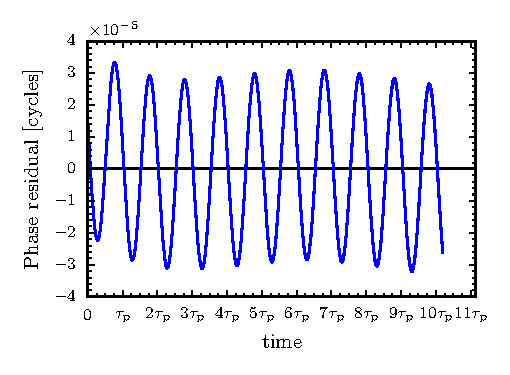
\includegraphics[width=0.5\textwidth]{NoSwitching.pdf}
}{%
    \caption{The phase residual for a minimal precession simulation with no
             switching event.}
  \label{fig: no switching}
}
\capbtabbox{%
  \begin{tabular}{ccl}
\multicolumn{3}{c}{Simulation parameters} \\
\hline
$\omega_0$  &=& 100 rad/s\\
$B_0$  &=& $10^{15}$ G \\
$\chi$  &=& 50$^{\circ}$ \\
$a_0$ &=& -0.78$^{\circ}$ \\
$\mathcal{A}_{\mathrm{EM}}$ &= & $23$
\end{tabular}

}{%
  \caption{}%
  \label{tab: NoSwitching properties}
}
\end{floatrow}
\end{figure}
Notably this minimal precession solution does show some precession with phase
residuals $\sim 10^{-4}$. This is because the spin-down torque produces a wobble
in the angular momentum vector and as a result the wobble angle is not truly
zero. In addition to this precessional wobble, there is also an inaccuracies
in the polynomial fitting which produces structure with a period equal to that
of the observation span.

We will now setup simulations of this `minimal precession` NS, and then
manually switch the torque. We choose a NS where the EM torque amplification
is important.

\subsection{Switching in the spin-down torque only}
We now consider manually switching the spin-down torque halfway though the
simulation, with no switch occurring in the anomalous component.
That is we set
\begin{align}
    t_{\mathrm{switch}} = \frac{\To}{2}, &&& \Ss = 0.4, &&& \Sa = 0.0,
\end{align}
such that halfway though the simulation the spin-down torque is reduced by a
fraction $0.4$ while the anomalous torque remains unaffected.

In Fig.~\ref{fig: switching without anom} we plot the phase residuals from
this simulation. In the top plot is the residual as calculated over the entire
observation period. We find a single periodic variation which is a direct result
of the sudden change in the spin-down rate. The precession features which existed
in the initial minimal precession are swamped by the larger variations due to
the switch. To study this simulation further,
in the lower plot we plot two residuals: the first is calculated
in the region $[0, t_{\mathrm{switch}}]$ and the second in $[t_{\mathrm{switch}}, \To]$,
the are marked by different colours.
Because the switch does not occur in either of these periods we can resolve the
free precession during each period and note that the precession modulation is
in fact smaller after the switch.
\begin{figure}[htb]
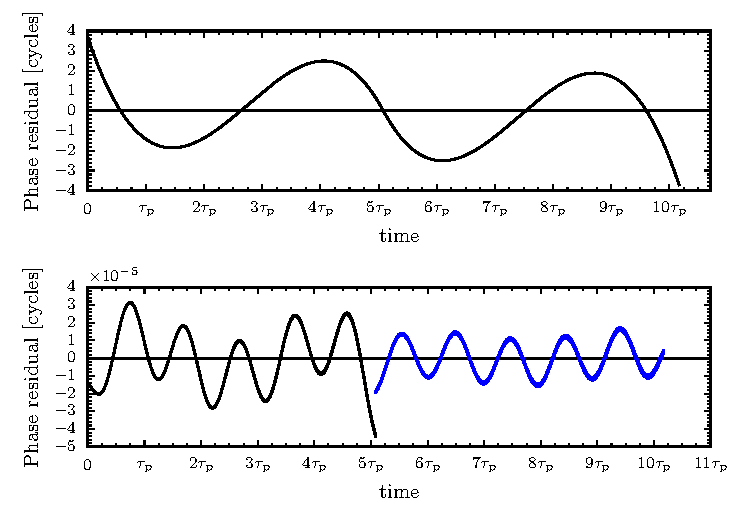
\includegraphics[width=.5\textwidth]{SwitchingWithoutAnomTorque}
\caption{Phase residuals for a simulation with a single switch in the spin-down
torque. In the top plot we show the residual calculated using the whole observation
time, in the bottom plot is the separate residuals calculated in the region before
and after the switch.}
\label{fig: switching without anom}
\end{figure}
This reduction in the size of modulations is because the precession is due to
the spin-down torque wobbling the angular moment vector. After the switch the
spin-down torque is reduced by a factor $\Ss$ and therefore the size of the
modulation is similarly reduced.

\subsection{Switching with the anomalous torque}
We now consider manually switching both the spin-down and anomalous torque
halfway though the simulation.  That is we set
\begin{align}
    t_{\mathrm{switch}} = \frac{\To}{2}, &&& \Ss = \Sa = 0.01
\end{align}

In a similar fashion to Fig.~\ref{fig: switching without anom} we show first
the total residual in the top plot of Fig.~\ref{fig: switching with anom}, and
then the individual residuals in the lower plot. Again the overall phase residual
shows strong periodic modulation resulting from the switch. In contrast to the
spin-down only switching, the amount of precession when considered before and
after the glitch now increases.

To understand this, recall that we begin with a minimal precession state, where
$\theta = \beta$ and the precession results from effect of the spin-down
torque.  After the switch, we have changed the size of the anomalous torque and
hence we have modified the effective rotating frame and the angle $\beta$. This
means that after the switch the wobble angle is no longer in a minimal
precession configuration.
This generates a significantly larger wobble angle producing a significant
increase in the phase residuals fitted in the post-switch period. The effect is
not observable when fitting to the entire simulation period since the switching
event remains dominant. In the next section we will calculate this new wobble
angle.

\begin{figure}[htb]
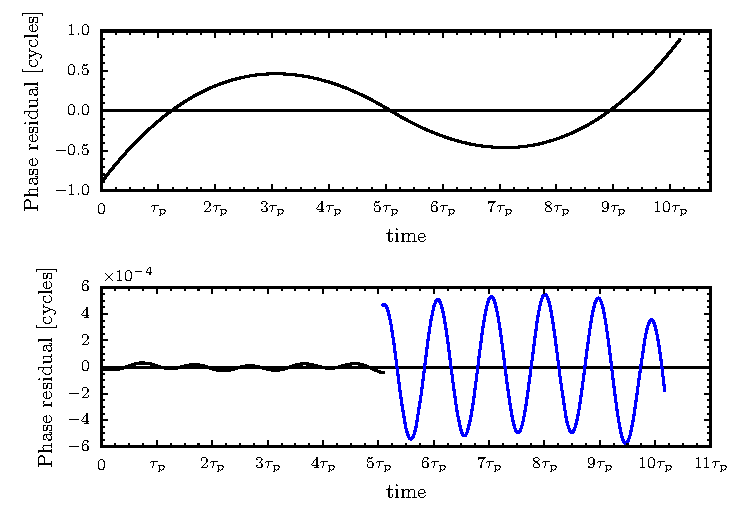
\includegraphics[width=.5\textwidth]{SwitchingWithAnomTorque} \caption{Phase
residuals for a simulation with a single switch in the spin-down and anomalous
torque. In the top plot we show the residual calculated using the whole
observation time, in the bottom plot is the separate residuals calculated in
the region before and after the switch.}
\label{fig: switching with anom}
\end{figure}

\subsubsection{Calculating the new wobble angle after a switch}
We now calculate the change in wobble angle and hence phase-residual variations
after switching a fraction of the anomalous torque.

The two-state switching changes the value of $\epsA$ according to
Eqn.~\eqref{eqn: epsA switch}, which in turn redefined the effective rotating frame
as defined in Sec.~\ref{sec: effective body frame}. A non-precessing NS at an
angle $\beta(\epsI, \epsA, \chi)$ will, after an anomalous torque switch by a fractional
amount $\Sa$, no longer be aligned with the rotating frame axis. This is
because the effective rotating frame will have shifted to $\beta' = \beta(\epsI,
\Sa\epsA, \chi)$. As a result, we should expect the previously
non-precessing NS to begin precessing after a torque switching event.

The NS will precess at the usual precession frequency in a cone  of half-angle
\begin{equation}
    \Delta\beta(\epsI, \epsA, \chi, \Sa)=|\beta - \beta'|,
\end{equation}
about the new effective body-frame axis.  The expression for $\Delta \beta$ is
not easily amenable to analytic calculation, but can easily be explored
graphically.  This is done in Fig.~\ref{fig: DeltaBetaPlot} for several choices
of $\Sa$. This illustrates that the new precession angle after a switch can be
as much as a few degrees although it tends to zero in the limit $\epsI \gg
\epsA$.
\begin{figure}[htb]
    \centering
    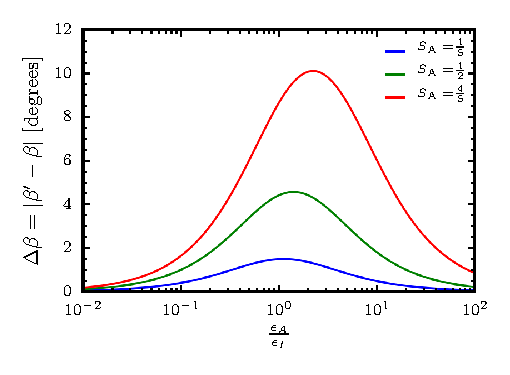
\includegraphics[]{DeltaBetaPlot}
    \caption{Illustrating the magnitude of the precession angle after switching
        due to the new rotation of the effective rotating frame. We plot the half-angle
        ($\Delta\beta$) of the precession cone as a function of the ratio
    $\epsA/\epsI$. Typically we expect real stars to have $\epsA < \epsI$.}
    \label{fig: DeltaBetaPlot}
\end{figure}

A simple application of this work is to apply our findings to PSR~B1828-11,
which was interpreted by \citet{Lyne2010} as undergoing switching with a fractional
change in the spin-down rate given by
\begin{align}
\frac{\Delta\dot{\nu}}{\dot{\nu}} = 0.0071
\end{align}
Manipulating Eqn.~\eqref{eqn: nudot switch}, we see that that
\begin{align}
|\Ss| = \frac{\Delta\dot{\nu}}{\dot{\nu}}
\end{align}
Using data from the ATNF catalogue \citep{ATNF}, B1828-11 has a frequency
$\nu = 2.47$~Hz, a spin-down rate $\dot{\nu}=-3.65\times10^{-13}$~Hz/s.
Rearranging Eqn.~\ref{eqn: spin-down of epsA} we then have
\begin{align}
\epsA^{B1828-11} = \frac{c}{8\pi R\nu^{3}}\dot{\nu} \approx 2.89 \times 10^{-11}
\end{align}

Now in this interpretation, $\epsI$ is unconstrained for B1828-11 since the
periodic modulations are assumed to be resulting from switching and not
precession. Nevertheless, we numerically maximise over $\epsI$ to find
\begin{align}
\Delta\beta_{\textrm{max}}(\epsI=2.89\times10^{-11}, \epsI=2.87\times10^{-11})
= 0.048 \textrm{ degs}
\end{align}
This is the new wobble angle which must occur every time B1828-11 undergoes a
switching event, if the switch also occurs in the anomalous torque. This
therefore provides a method to probe how the switching mechanism works by
looking at timing residuals in the post-switch timing data to check for
any signs of precession.

\section{Conclusions}

In this chapter we have developed a method to simulate observable properties of
neutron stars by evolving the governing system of ODEs. These equations
\eqref{eqn: ODEs} contain both the components of the spin vector in the
rotating frame and the Euler rotation angles required to transform from
the rotating frame to the inertial frame. This step is important since it is in
this reference frame that observers see the peculiar features of precession.

We developed an intuitive model for how the magnetic dipole, along which EM
radiation is emitted, moves in the inertial frame. Comparing with analytic
models where possible, we showed how the calculate from the motion of the
dipole the evolution of the stars timing properties (the phase, frequency, and
spin-down rate) and how to calculate features of the beam shape such as the
beam-width.

Finally, we used the phase residuals to investigate the effect of a simple torque
switching model in which the components of the torque instantaneously change.
This was done to model, in a simple way, the magnetospheric switching which is
proposed by \citet{Lyne2010} as an explanation of the periodic modulation of
B1828-11. Our numerical model is ideally suited to this task as it captures the
complicated feedback between precession and the changing torque.
A future application of this model is to link the switching to the precessional
phase in a probabilistic way as proposed by \citet{Jones2012}. In this way
precession provides the clock to the switching. We feel that, by virtue of
being probabilistic, such a system will display stochastic resonance as first
described by \citet{Cordes2013}.

\biblio

\end{document}
